% 中文摘要      I_chabstract.tex
% 英文摘要      II_enabstract.tex
% 誌謝          III_acknowledge.tex

% 主程ot                00_masterthesis.tex
% 緒論                  01_introduction.tex
% 背景知識與相關文獻    02_relatedwork.tex
% 問題分析              03_analysis
% 研究方法              04_method.tex
% 實驗與結果分析        05_experiment.tex
% 結論                  06_conclusion.tex
% 附錄                  07_appendix.tex

% clean.bat 為清除、複製檔案於 C:\xtemp 使用。
% IEEEtran.sty 為文獻格式必須檔。
% *.bib 為文獻檔
%%%%%%%%%%%%%%%%%%%%%%%%%%%%%%%%%%%%%%%%%%%%%%%%%%%%%%%%%%%%%%%%%%%%%%%%%%%%%%%%%%%%%%%%%%%%%%%%%%%%
\documentclass[12pt,oneside,openany,a4paper,draft=FALSE]{book}

% 套件集
%\usepackage[left=3cm,top=3cm,nohead]{geometry}
%\usepackage[total={15cm,24cm}, top=35mm, left=36mm, includefoot]{geometry}
\usepackage[total={15cm,24cm}, top=30mm, left=30mm, includefoot]{geometry}  %版面格式

%首行縮排
\usepackage{indentfirst}
\usepackage{times}
\usepackage{titlesec}
\usepackage{caption}
\usepackage{comment}
\usepackage{bm}
%\usepackage[usenames,dvipsnames]{color}     %自訂文字顏色
\usepackage{graphicx,subfigure,float}       % 所有圖片均為浮動狀態,可為圖片編碼
\usepackage{tikz}
\usepackage{amsmath,amssymb}                % 數學式
%\usepackage{color,colortbl,lettrine,wrapfig}
%\usepackage{epstopdf} %EPS轉PDF功能
%\usepackage[bookmarks=false,colorlinks=true,breaklinks=true]{hyperref} %PDF書籤與連結功能
\usepackage[numbered]{bookmark} %PDF書籤與連結功能
\usepackage[titletoc]{appendix}
%\usepackage{breakurl}

%註腳不縮排
\usepackage[bottom,hang,flushmargin]{footmisc}

% 文獻套件
\usepackage[square,numbers]{natbib} %中英文文獻
%\usepackage{natbib}
\usepackage{bibentry}
%\usepackage{biblatex}
%\usepackage[notocbib]{apacite}     % use APA citation
%\usepackage{IEEEtran}   %IEEE文獻
\usepackage[notindex,nottoc,notlot,notlof]{tocbibind}

\usepackage{longtable}
\usepackage{url}
\usepackage{wallpaper}     % 浮水印


% 表格套件
\usepackage{array}
\usepackage{fancyhdr}
\usepackage{rotating}   % 旋轉表格,將某頁版面由直排轉為橫排,適合用於旋轉占滿一頁的表格或圖形
\usepackage{booktabs}
%\usepackage{graphicx,floatrow}

% 數學
\usepackage{amsthm}     % 排版數學文稿的定理與定義
\usepackage{amsmath}
\usepackage{enumerate}  % 條列項目 (阿拉伯數字編號)

%% 中文專用
\usepackage{fontspec} %加這個就可以設定字體
\usepackage{ctex} %讓中英文字體分開設置

\usepackage{mathptmx}
\usepackage[T1]{fontenc}


%畫圖套件
\usepackage{mathrsfs}
\usepackage{pgfplots}
\pgfplotsset{compat=1.15}
\usetikzlibrary{arrows}

%-----

% 設定『目錄』名稱
\renewcommand{\contentsname}{目錄}
\renewcommand{\listfigurename}{圖目錄}
\renewcommand{\listtablename}{表目錄}
%\renewcommand{\appendixtocname}{附錄}   % if \appendix  is used.
\renewcommand{\appendixname}{附錄}   % if \appendix  is used.
\renewcommand{\tablename}{表}
\renewcommand{\figurename}{圖}
\renewcommand{\bibname}{參考文獻}

\hypersetup{
    bookmarks=true,         % show bookmarks bar?
    colorlinks=true,        % false: boxed links; true: colored links
    linkcolor=black,          % color of internal links (change box color with linkbordercolor)
    citecolor=black,          % color of links to bibliography
    filecolor=cyan,         % color of file links
    urlcolor=magenta        % color of external links
}

%\newcommand{\img}{C:/Dropbox/ntpu_thesis/plot/}%如果所有圖檔存放在其他地方,先定義位置

\pagestyle{fancy}
\fancyhf{}
\renewcommand{\chaptermark}[1]{\markboth{\thechapter .\ #1}{}}  % 去除章編號前後的字
\titleformat{\chapter}[display]{\center\LARGE\sf}{第\ \thechapter\ 章}{0.2cm}{}  %設計章節標題式樣,標題置中
\titlespacing{\chapter}{0pt}{-50pt}{25pt}   %設計章節標題式樣,控制間距
%\fancyhead[RO,RE]{\leftmark}   %章節標題於頁眉/頁足上
\fancyfoot[CO,CE]{\thepage}

\renewcommand{\headrulewidth}{0pt}  % 頁眉下方的橫線
%\renewcommand{\footrulewidth}{0pt} % 設定頁首多一條粗細是 0.4 pt 的水平線

% 設定itemize符號
\renewcommand{\labelitemi}{$\bullet$}
\renewcommand{\labelitemii}{$\circ$}

%設定英文字型,不設的話就會使用預設的字型
\setmainfont{Times New Roman}

% 設定中文字體
\setCJKmainfont{標楷體} %設定中文為系統上的字型,而英文不去更動,使用原TeX字型
%\setCJKmainfont{cwTeXKai}
\XeTeXlinebreaklocale "zh"
\XeTeXlinebreakskip = 0pt plus 1pt %這兩行一定要加,中文才能自動換行


\renewcommand{\baselinestretch}{1.25}   %依照文章預設行距增加為 1.25倍(不同字型大小行距值,加大為1.25倍)

% 以下是目錄章節後面打點格式的設定:http://vardesa.blog.hexun.com.tw/58537832_d.html
\makeatletter
\def\@bfdottedtocline#1#2#3#4#5{%
\ifnum #1>\c@tocdepth \else
\vskip \z@ \@plus.2\p@
{\leftskip #2\relax \rightskip \@tocrmarg \parfillskip -\rightskip
\parindent #2\relax\@afterindenttrue
\interlinepenalty\@M
\leavevmode \bfseries
\@tempdima #3\relax
\advance\leftskip \@tempdima \null\nobreak\hskip -\leftskip
{#4}\normalfont\nobreak
\leaders\hbox{$\m@th
\mkern \@dotsep mu\hbox{.}\mkern \@dotsep
mu$}\hfill
\nobreak
\hb@xt@\@pnumwidth{\hfil\normalfont \normalcolor #5}%
\par}%
\fi}
\renewcommand*\l@chapter{\@bfdottedtocline{0}{0em}{1.5em}}
\makeatother

% 定義『各章節標題、圖表、頁尾註記』字型

\theoremstyle{plain}   % 排版格式,{plain}:最醒目格式
\newtheorem{thm}{定理}  % 將 Theorem 改為國字「定理」
\newtheorem{thmm}{定義}


%
%   調整內縮長度(依據學校規定與不同版面、字型調整)
%
\parindent=0.85cm
%% 修改中文標題與格式定義
\date{2013.9.18}    %版本日期

%%%%% 論文開始 %%%%%
\begin{document}

%%  封面
%% 封面頁
\fontsize{24}{20pt}\selectfont
\thispagestyle{empty}


\vspace*{1cm}

\vspace*{\fill}
\begin{center}
	\fontsize{24}{18pt}
	%\LARGE 筆記 \\

\end{center}
\vspace*{\fill}



\vspace*{0.5cm}

\begin{center}
	\fontsize{24}{18pt}
	\LARGE 作者:X X X   撰\\
\end{center}

\vspace*{0.5cm}


\newpage


%%
%%\CenterWallPaper{0.17}{graphs/logo/logowatermark.eps} %浮水印
%===============================================================
%%%%%%%%%%%%%%%%---------- 中文摘要
\frontmatter % 羅馬文頁碼


%%  目錄
\newpage
%%\newpage
\fontsize{12}{18pt}\selectfont
%%  目錄
\phantomsection
\addcontentsline{toc}{chapter}{目錄} %手動加入目錄文字
\tableofcontents
\newpage
%%  圖目錄
%%\phantomsection
%%\addcontentsline{toc}{chapter}{圖目錄} %手動加入目錄文字
%%\listoffigures
%%\newpage
%%%%  表目錄
%%\phantomsection
%%\addcontentsline{toc}{chapter}{表目錄} %手動加入目錄文字
%%\listoftables
%%\newpage


%%%%%%%%%%%%%%%%%%%% 碩士論文內文開始 %%%%%%%%%%%%%%%%%%%%

%%%%%%%%%%%%%%%%---------- 開始章節
\cleardoublepage
\mainmatter % 阿拉伯文頁碼
\fontsize{12}{21pt}\selectfont

%%  第一章
%\chapter{緒論}
\label{chapter:intro}
\section{研究背景與動機}
\label{sec:background}
    \subsection{子章節一}
        字章節一段落一,字章節一段落一,字章節一段落一,字章節一段落一,
        字章節一段落一,字章節一段落一,字章節一段落一,字章節一段落一,
        字章節一段落一,字章節一段落一,字章節一段落一,字章節一段落一,
        字章節一段落一,字章節一段落一,字章節一段落一,字章節一段落一,
        字章節一段落一,字章節一段落一,字章節一段落一。

        字章節一段落二,字章節一段落二,字章節一段落二,字章節一段落二,
        字章節一段落二,字章節一段落二,字章節一段落二,字章節一段落二,
        字章節一段落二,字章節一段落二,字章節一段落二,字章節一段落二,
        字章節一段落二,字章節一段落二,字章節一段落二,字章節一段落二,
        字章節一段落二,字章節一段落二,字章節一段落二,字章節一段落二,
        字章節一段落二,字章節一段落二,字章節一段落二,字章節一段落二,
        字章節一段落二。

        例如現有的系統有\cite{GoogleComputeEngine}、\cite{AmazonEC2}等等,
        另外\cite{GoogleApps}是以○○○技術來達成。

        ○○系統結構如示意圖\ref{fig:this_system}
        \begin{figure}[htbp]
            \centerline{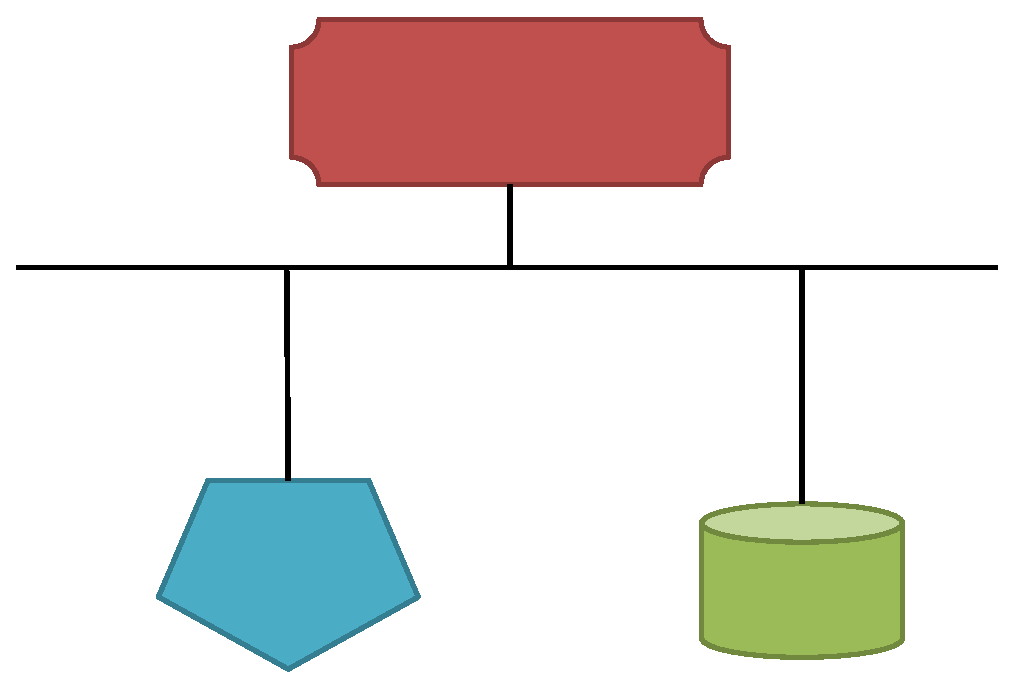
\includegraphics[height=5cm]{graphs/introduction/this_system.eps}}
            \caption{○○示意圖}
            \label{fig:this_system}
        \end{figure}

    \subsection{子章節二}
        字章節二,字章節二,字章節二,字章節二,字章節二,
        字章節二,字章節二,字章節二,字章節二,字章節二,
        字章節二,字章節二,字章節二,字章節二,字章節二,
        字章節二,字章節二,字章節二,字章節二,字章節二,
        字章節二,字章節二,字章節二,字章節二,字章節二,
        字章節二,字章節二,字章節二,字章節二,
        ○○○如圖~\ref{fig:types_comparison}所示。
        \begin{figure}[!t]
            \begin{center}
                \begin{tabular}{ccccccccccccc}
                    \subfigure[類型A]{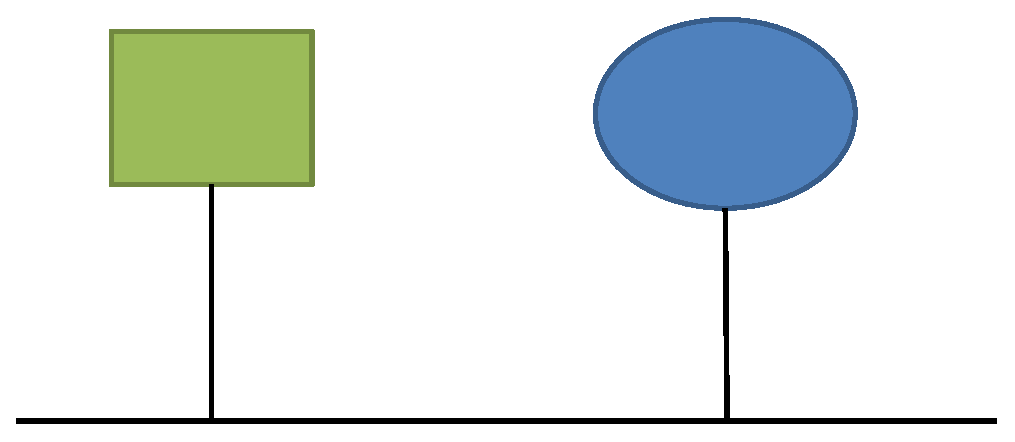
\includegraphics[height=2.4cm]{graphs/introduction/typeA.eps}\label{fig:typeA} } \par &
                    \subfigure[類型B]{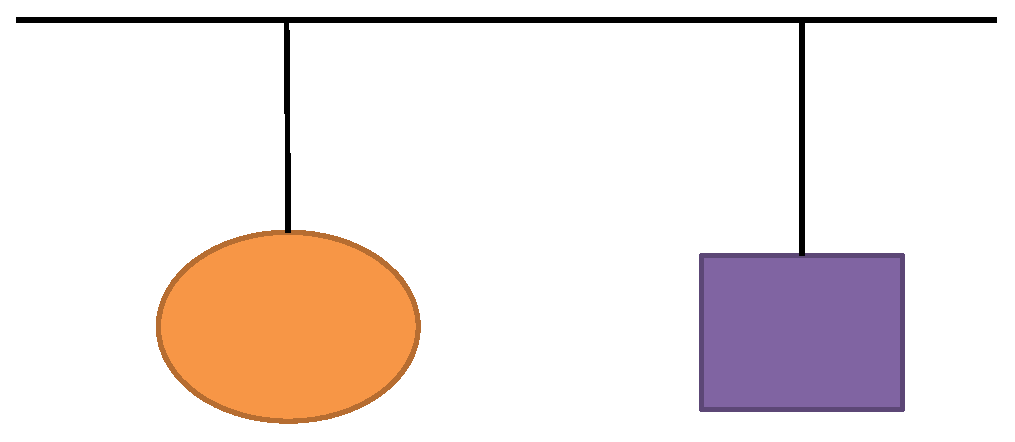
\includegraphics[height=2.4cm]{graphs/introduction/typeB.eps}\label{fig:typeA} } \par \\
                \end{tabular}
                \caption{○○○比較}
                \label{fig:types_comparison}
            \end{center}
        \end{figure}

\section{○○○問題與處理機制}
    問題與機制,問題與機制,問題與機制,問題與機制,
    問題與機制,問題與機制,問題與機制,問題與機制,
    問題與機制,問題與機制,問題與機制,問題與機制,
    問題與機制,問題與機制,問題與機制,問題與機制,
    問題與機制。

    %要被單行註解的文字。

\begin{comment}
    要被區塊註解的文字,要被區塊註解的文字,要被區塊註解的文字,
    要被區塊註解的文字,要被區塊註解的文字,要被區塊註解的文字,
    要被區塊註解的文字,要被區塊註解的文字,要被區塊註解的文字,
    要被區塊註解的文字,要被區塊註解的文字,要被區塊註解的文字,
    要被區塊註解的文字,要被區塊註解的文字,要被區塊註解的文字,
    要被區塊註解的文字,要被區塊註解的文字。
\end{comment}

\section{研究動機與目的}
    動機與目的,動機與目的,動機與目的,動機與目的,
    動機與目的,動機與目的,動機與目的,動機與目的,
    動機與目的,動機與目的,動機與目的,動機與目的,
    動機與目的,動機與目的,動機與目的,動機與目的,
    動機與目的,動機與目的,動機與目的,
    細節如表\ref{tab:mytitle1}。
    \begin{table}[!t]
        \centering
        \caption{表格標題1}
        \label{tab:mytitle1}
        % Table generated by Excel2LaTeX from sheet 'table_01'
\begin{tabular}{rr}
\toprule
Title & Values \\
\midrule
A     & 1612 \\
B     & 256 \\
C     & 30 \\
D     & 7 \\
E     & 3 \\
\bottomrule
\end{tabular}%

    \end{table}

    \begin{enumerate}
        \item
        列舉一。
        %
        \item
        列舉二。
        %
        \item
        列舉三。
        %
    \end{enumerate}

\section {研究方法與論文架構}
    研究方法與論文架構,研究方法與論文架構,研究方法與論文架構,
    研究方法與論文架構,研究方法與論文架構,研究方法與論文架構,
    研究方法與論文架構,研究方法與論文架構,研究方法與論文架構,
    研究方法與論文架構。

    \begin{itemize}
        \item
        項目一。
        %
        \item
        項目二。
        %
        \item
        項目三。
        %
        \item
        項目四。
    \end{itemize}

    流程圖如\ref{fig:ResearchFlowChart}。
    \begin{figure}[htbp]
        \centering
        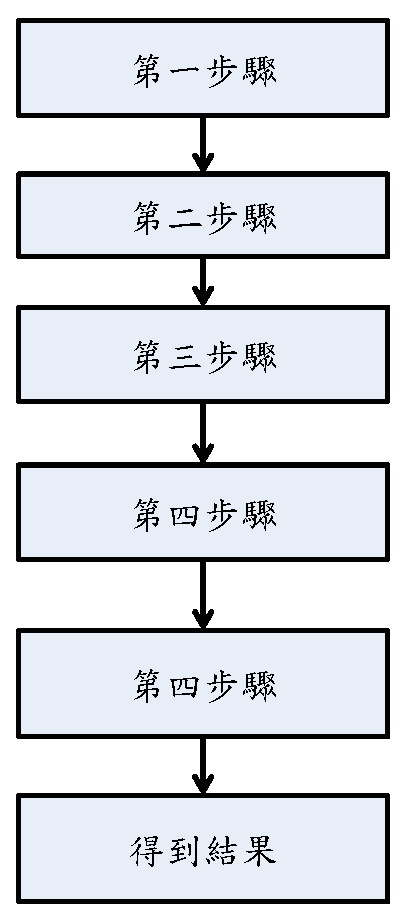
\includegraphics[height=8cm]{graphs/introduction/ResearchFlowChart.eps}
        \caption{研究進行流程圖}
        \label{fig:ResearchFlowChart}
    \end{figure}




% 	PCA
\chapter{Principal Component Analysis}
\label{chapter:pca}
\section{簡介}
\label{sec:introduction}


在機器學習中,資料的特徵(維度)數往往會影響模型的訓練效果,特徵太少可能所包含的資訊量太少,在進行模型訓練時,無法順利將資料進行正確的分類,所以會僅可能收集與資料集相關的特徵。
但當資料的特徵多到一定的程度時,卻會因爲所包含的資訊太多,導致訓練出來的模型過擬合的現象,以至於分類器的效果不增反減,這種現象我們稱爲「curse of dimensionality」,如圖\ref{fig:CurseOfDimesionality}所示。所以在資料特徵過多的情況下,會進行資料降維,盡可能的減少模型發生過擬的現象,增加模型的訓練效果。

主成份分析(Principal Component Analysis,PCA),是一種非監督式的資料降維演算法,
主要是分析數據集中的一系列的主成份,將原本的數據集轉換到一個新的數據集。
其中在這一系列的主成份中,第一主成份,就是能在特徵空間中,找出一個投影向量,使得這些資料的投影點能有最大的變異數,而第二主成份則是能找到第二大變異數的投影向量,以此類推。




\begin{figure}[h]
	\centering
	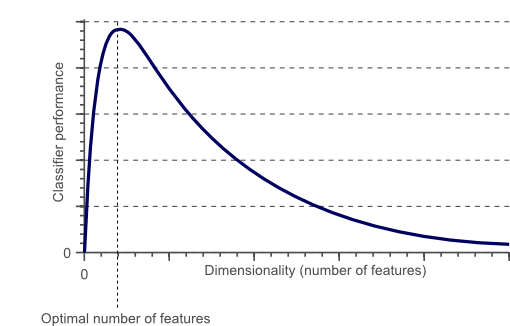
\includegraphics[height=5cm]{./pic/NZgacRXF.png}
	\caption{curse of dimensionality 示意圖}
	\label{fig:CurseOfDimesionality}
\end{figure}

\section{相關參數與實例說明}
為了更簡單理解這個演算法的數學意義,以下舉一個例子說明:

\subsection{相關參數}
\begin{itemize}
	\item
		\(\mathbf{x}\) 為原資料點, \(\mathbf{\overline{x}}\) 表示原資料的均值。
	\item
		\(z\) 為過投影後資料點的值,\(\overline{z}\)則為投影後的均值。 
	\item
	      \(\mathbf{S}\) 資料變異量。而 \(\mathbf{{S}'}\)是資料經過投影後的變異量量。
	\item
	      \(\mathbf{v}\) :投影向量。
\end{itemize}


\subsection{實例說明}

\begin{itemize}
	\item
	      圖\ref{fig:PcaDemostrate}為一個具有兩個維度的資料分佈圖。


	      \begin{figure}[h]
		      \centering
		      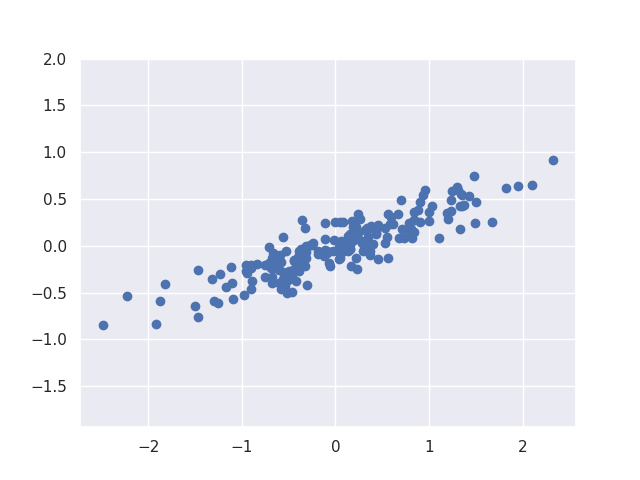
\includegraphics[width=9cm]{pic/pca_demostrate.png}
		      \caption{二維資料}
		      \label{fig:PcaDemostrate}
	      \end{figure}


	      %
	\newpage
	\item
	      而PCA這個演算法的目的就是希望從這些資料點中如圖\ref{fig:PcaVectorToFind},找出投影向量,使得這些資料點投影在這些向量上後具有最大的變異數\footnote{\noindent 變異數:為對數據的變異程度的衡量,常用來量測資料分散程度之指標值,變異數其定義為 \(\sigma^2=\frac{{}\sum^{N}_{i}(x_i-\mu )^2}{N}\) }。
	      \begin{figure}[h]
		      \centering
		      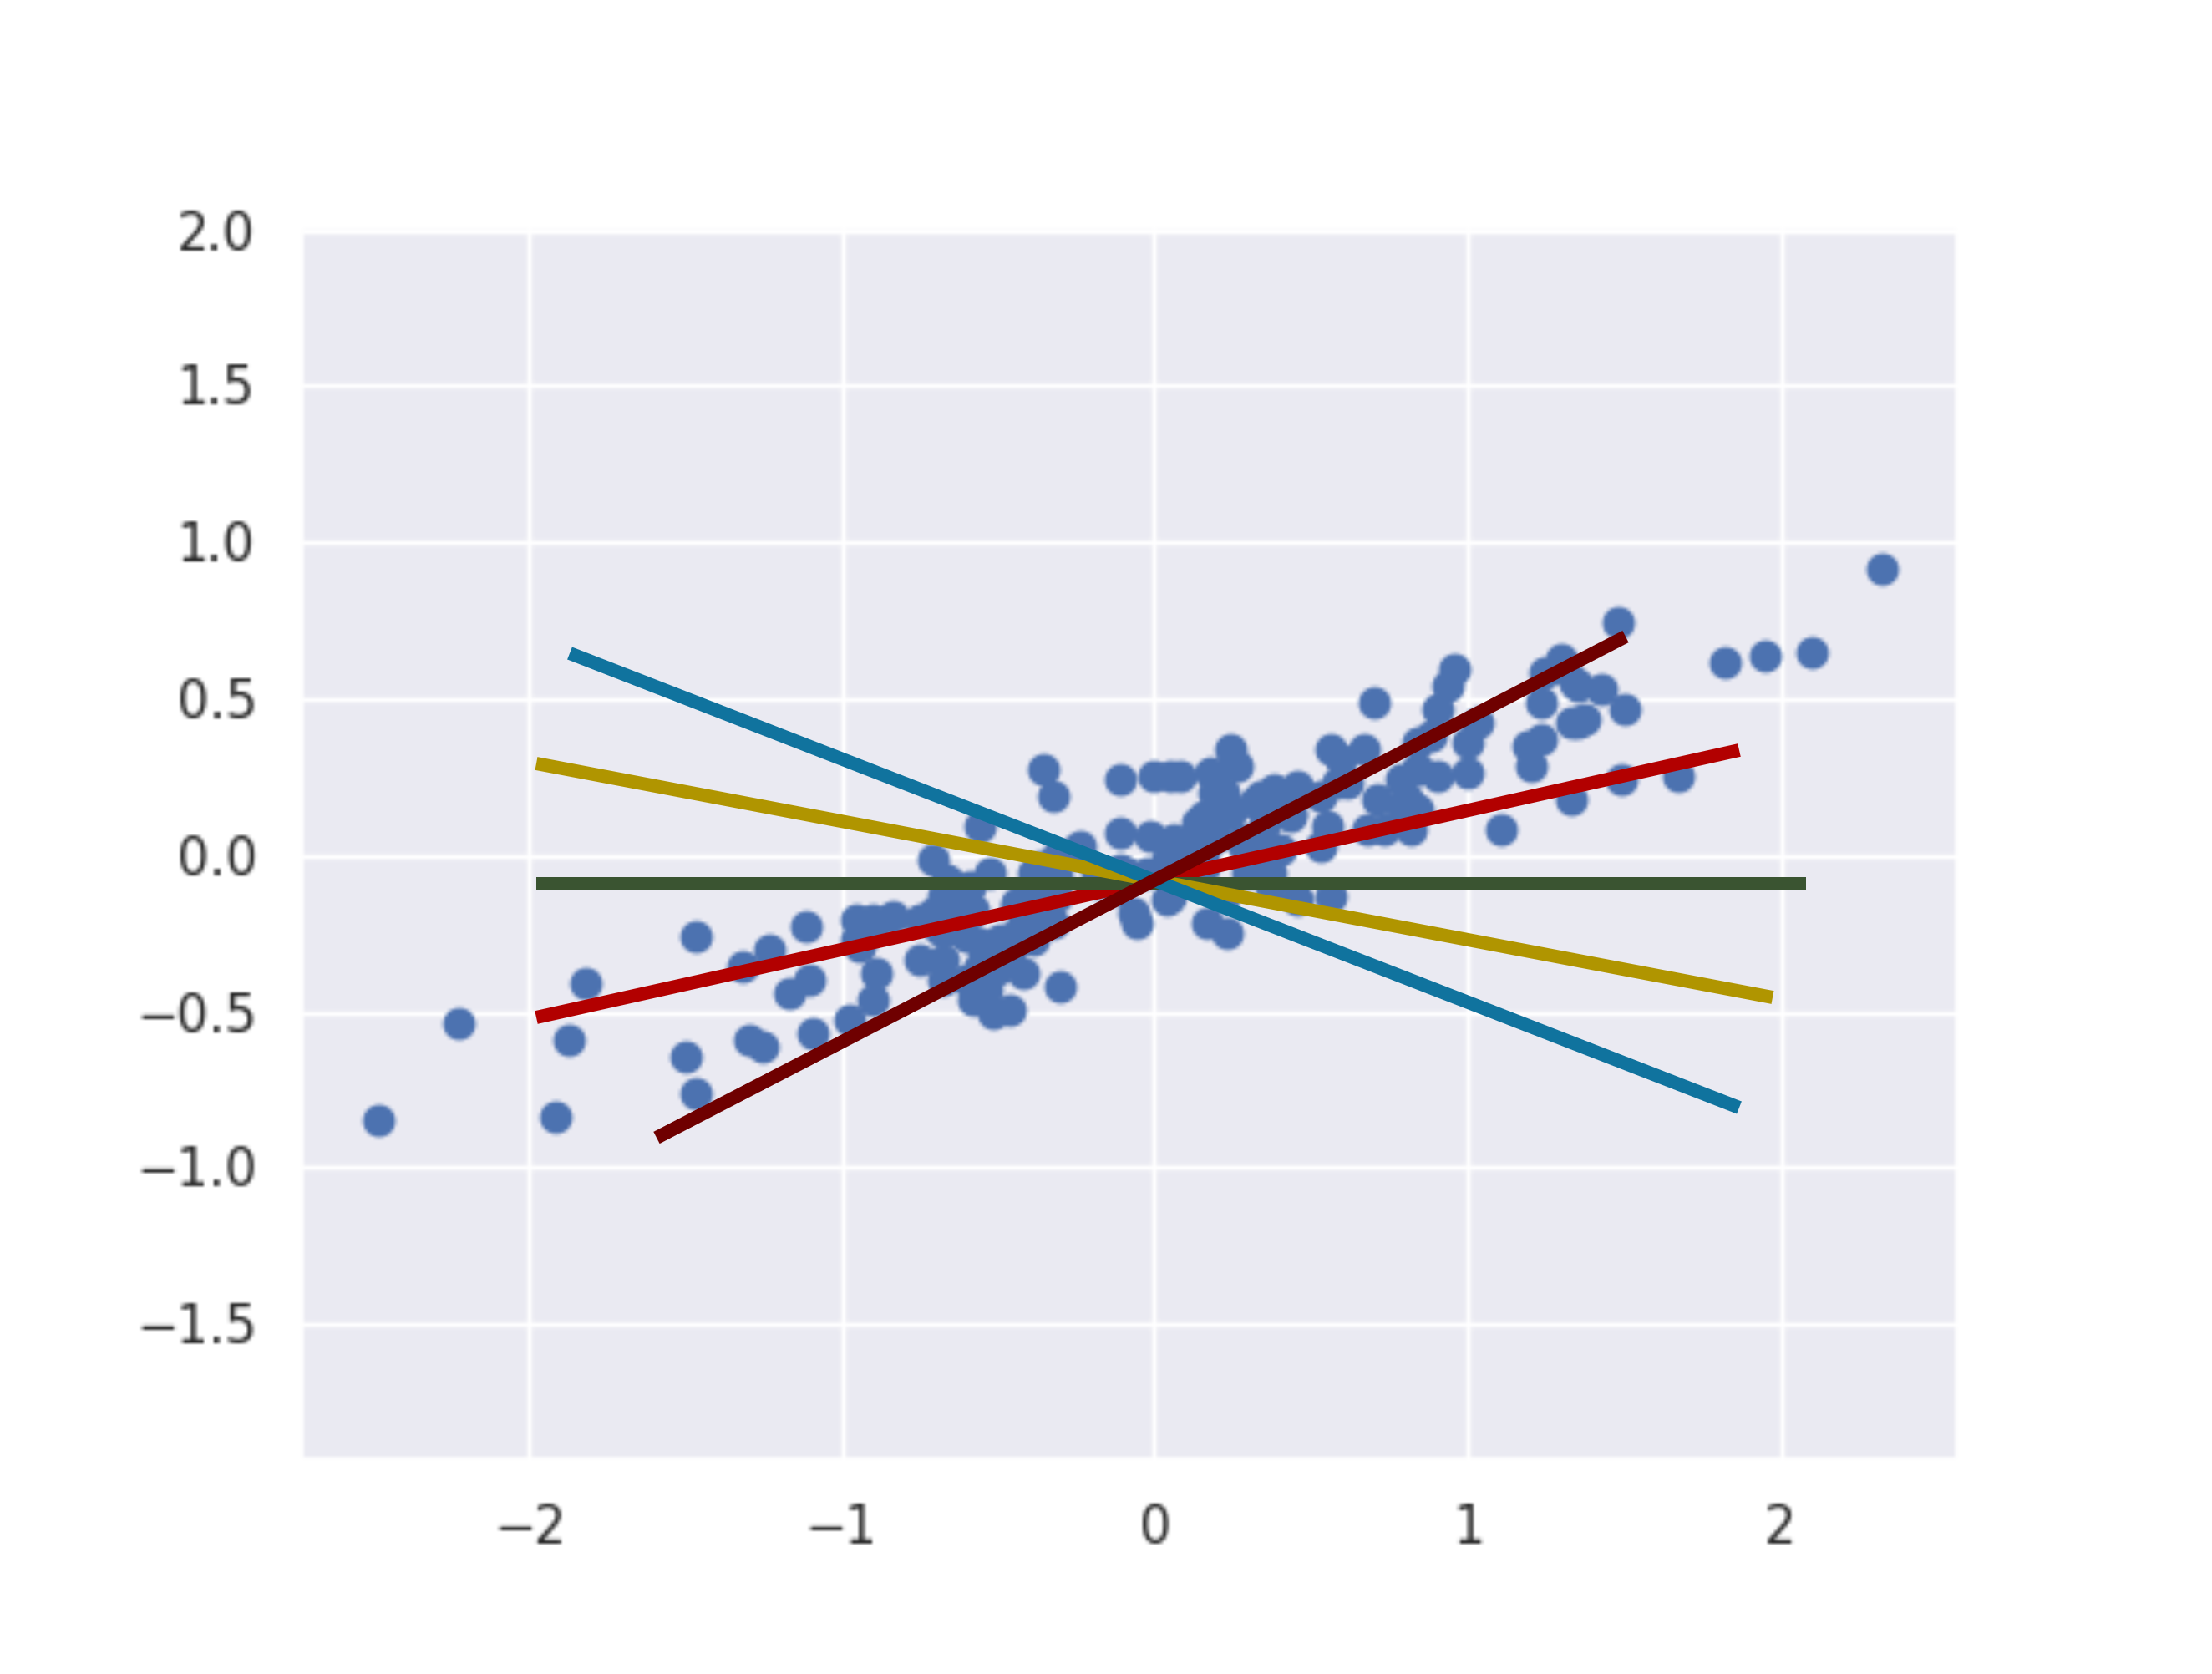
\includegraphics[width=9cm]{./pic/iVu9zQYG.png}
		      \caption{}
		      \label{fig:PcaVectorToFind}
	      \end{figure}
	      %
	\item
		式(\ref{eqn:ProjectData})為投資料投影的公式,圖 \ref{fig:VectorProject}為部分資料集於兩向量上的投影示意圖。 
		\begin{equation}
			\label{eqn:ProjectData}
			 z = v^Tx
		\end{equation}


	      \begin{figure}[H]
		      \begin{center}
		      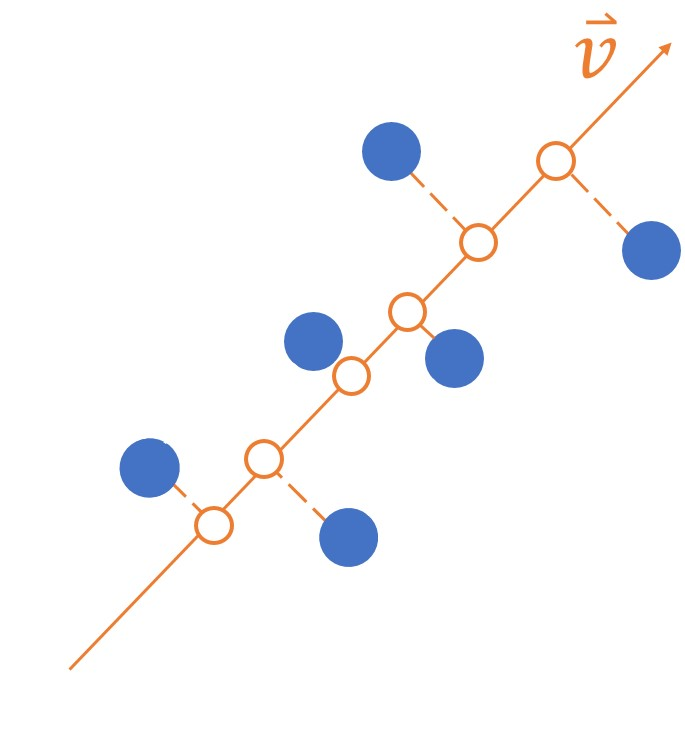
\includegraphics[width=5cm]{pic/pca_project_1.jpg}
			      \caption{部分資料集投影於向量上示意圖}
			      \label{fig:VectorProject}
		      \end{center}
	      \end{figure}

	\item
		式(\ref{eqn:VarianceWithProject})為資料進過投影後的變異量運算式。圖 \ref{fig:PcaProjectAll}為部分資料集於兩向量上的投影示意圖,可以發現,資料於\(\vec{v}\)上的投影擁有較大的變異數。 

	      \begin{equation}
		      \label{eqn:Variance}
		      \mathbf{S}  =\sum_{i=1} (\mathbf{x_i} - \mathbf{\overline{x}})(\mathbf{x_i}-\mathbf{\overline{x}})^T
	      \end{equation}

	      \begin{equation}
		      \label{eqn:VarianceWithProject}
		      \begin{aligned}
				  \mathbf{{S}'} &=\sum_{i=1} (z_i - \overline{z})(z_i-\overline{z})^T 
							  \\&=\mathbf{\sum_{i=1} (v^Tx_i - v^T\overline{x})(v^Tx_i-v^T\overline{x})^T}
							  \\&=\mathbf{v^T(\sum_{i=1} (x_i - \overline{x})(x_i-\overline{x})^T)v}
							  \\&=\mathbf{v^TSv}
		      \end{aligned}
	      \end{equation}



	      \begin{figure}[H]
		      \centering
		      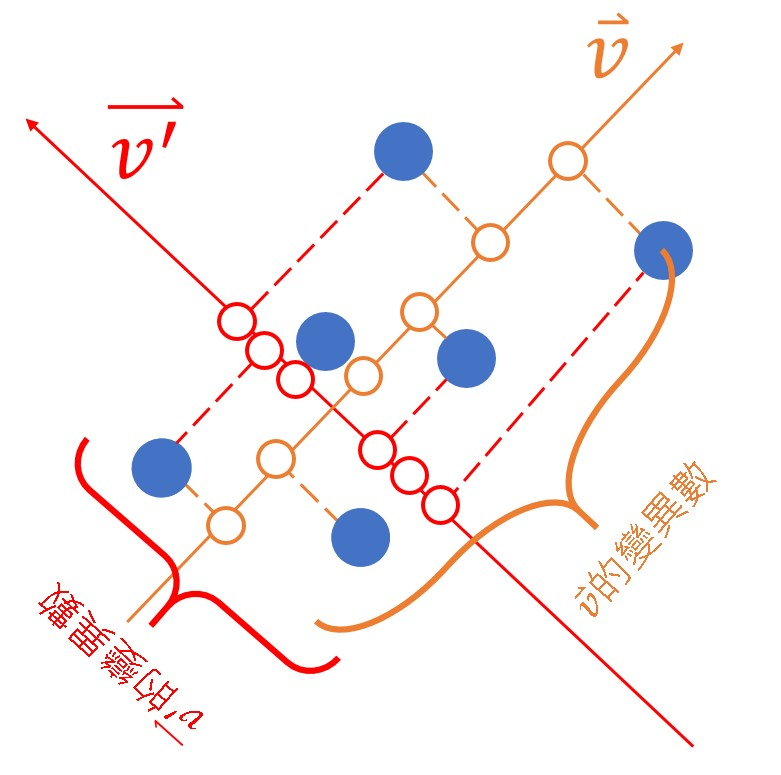
\includegraphics[width=6cm]{pic/pca_project_all.jpg}
			  \caption{\(\vec{v}\) 與\(\vec{{v}'}\)的變異數比較} 
		      \label{fig:PcaProjectAll}
	      \end{figure}
	      
	      %
	\item
		在PCA中,就是找出一個投影向量 \(\mathbf{v}\) ,使得所有資料經過投影能有最大的變異數,如式(\ref{eqn:MaxProjetVector})。

		%%\begin{equation}
		%%	\label{eqn:MaxProjetVector}
		%%	\mathbf{v} = arg max\  \mathbf{v^Tsv}			
		%%\end{equation}

		\begin{equation}
			\label{eqn:MaxProjetVector}
		\mathbf{v} = \underset{\mathbf{v}\in R^d ,\mathbf{||v||_2}=1}{argmax}\  \mathbf{v^tsv}			
		\end{equation}


		\newpage
	\item
		經過PCA的計算之後,我們可以得到比較有代表性的兩個特徵成份,較長的為PC1,較短的為PC2,如圖\ref{fig:Pc1AndPc2}所示,而變異量的值分別為0.7625與0.0184 。


	      \begin{figure}[H]
		      \centering
		      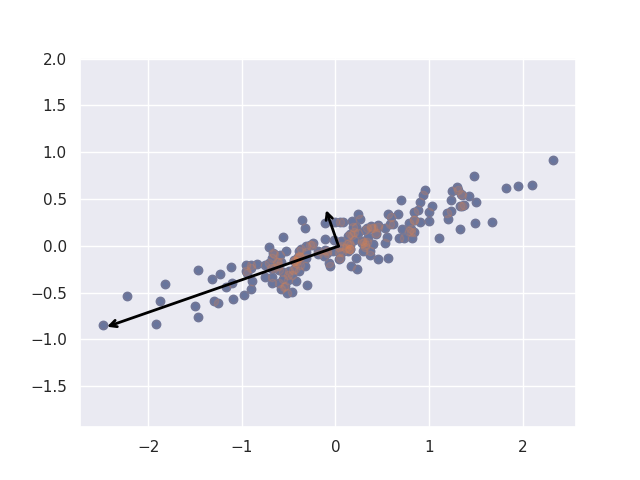
\includegraphics[width=9cm]{pic/pca_with_pca_axis.png}
		      \caption{PC1與PC2在原始資料上}
		      \label{fig:Pc1AndPc2}
	      \end{figure}


	\item
	圖\ref{fig:PcaTransform}為資料集經過PCA轉換的結果,橫軸為PC1,縱軸為PC2,能從圖中與上面得到的變異量發現,PC1所函概的資訊足以代表整個資料集。進而將原本二維的資料,轉換成一維,利用PC1作為模型訓練的輸入。


	      \begin{figure}[H]
		      \centering
		      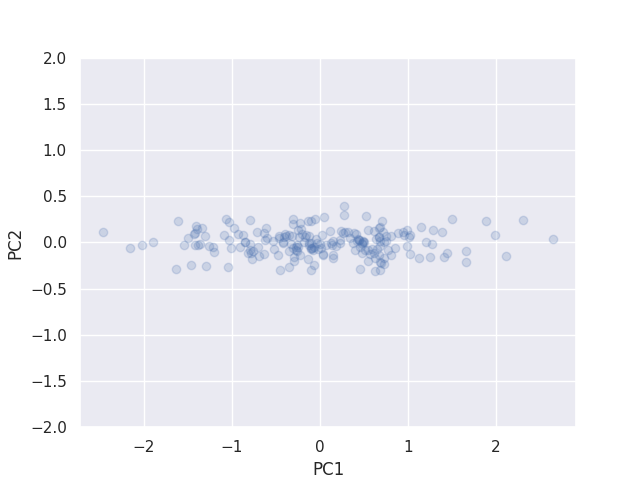
\includegraphics[width=9cm]{pic/pca_transform.png}
		      \caption{資料經過PCA轉換的結果}
		      \label{fig:PcaTransform}
	      \end{figure}

\end{itemize}


\section {結論}
從以上的舉例中,可以發現,經由PCA的轉換,我們可以分析出對於整個資料集最具代表性的成份,作為後序模型訓練的輸⼊資料。
也許二維的資料可能沒那麼明顯,但如果是影像資料(通常是具有高維度的資料),除了能夠有效的進行資料降維,提取影像中重要的特徵,還能因為維度的減少進而提高分類的運算速度。



% 	LDA
\chapter{Linear Discriminant Analysis}
\label{chapter:lda}
\section{簡介}
\label{sec:LdaIntroduction}




%Linear Discriminant Analysis(LDA),是一種降維演算法,但與前一節提到的PCA有些許的不同,這個演算法屬於一種「監督式」的學習法,所以在進行演算法的運算時,須考慮資料的類別。

線性區別分析(Linear Discriminant Analysis,LDA),屬於一種「監督式」的降維演算法,所以在進行演算法運算時,須考慮資料的類別。
前一小節提到PCA是希望能在特徵空間中找到一個向量,使得資料的投影點,彼此之間的變異數越大越好。而LDA則是希望能夠找到一個投影向量,使得組內的離散程度越小越好,與組間的離散程度越大越好。




\section{相關參數與實例說明}
為了更簡單理解這個演算法的數學意義,以下舉一個例子說明:


\subsection{相關參數}

\begin{itemize}
	\item
	      \(\mathbf{S_w}\) 為組內離散程度矩陣,不同類別中的資料變異量總合。而 \(\mathbf{{S_w}'}\)是經過投影後的組內離散程度矩陣。
	\item
	      \(\mathbf{S_b}\) 為組間離散程度矩陣,表示兩兩類別之間群心的變異量的總合。\(\mathbf{{S_b}'}\) 為投影後的組間離散程度矩陣。
	\item
	      \(u\) :所有資料均值。
	\item
	      \(u_i\) :第i類資料均值。
	\item
	      \(x_i\) :第i筆資料。
	\item
	      \(n_i\) :屬於i類的資料個數。
	\item
	      \(w\) :投影軸。
\end{itemize}

\subsection{實例說明}
\begin{itemize}
	\item
	      圖\ref{fig:LdaDemostrate}為一個具有兩個維度的資料分佈圖,分別有黃、藍、灰三類。
	      \begin{figure}[h]
		      \centering
		      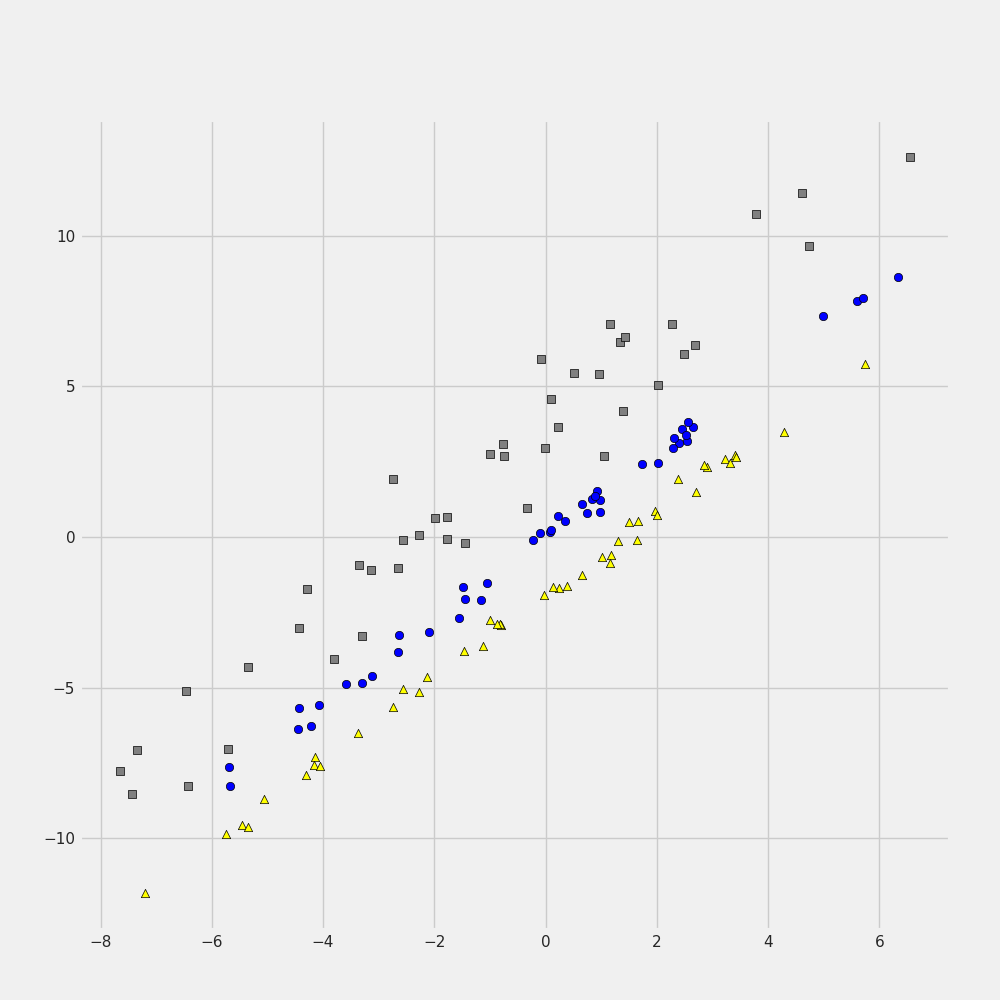
\includegraphics[width=6cm]{pic/lda_dataset.png}
		      \caption{二維資料}
		      \label{fig:LdaDemostrate}
	      \end{figure}


	      %
	\item
	      首先,由式(\ref{eqn:LdaWithin})計算不同類別的變異數總合 \(\mathbf{S_w}\)。並由式(\ref{eqn:LdaWithinTransform})計算經過投影後的組內離散矩陣 \(\mathbf{{S_w}'}\)。

	      %%由式(\ref{eqn:LdaWithinTransform})計算經過「投影後」的組內離散矩陣 \(\mathbf{{S_w}'}\)。其中 \(\mathbf{S_w}\) 為不同類別的變異數總合。

	      \begin{equation}
		      \label{eqn:LdaWithin}
		      \mathbf{S_w}  =\sum_{i=1}^{c} \sum^{}_{x_k\in class}  (x_k - u_i)(x_k-u_i)^T
	      \end{equation}

	      \begin{equation}
		      \label{eqn:LdaWithinTransform}
		      \begin{aligned}
			      \mathbf{{S_w}'} & =\sum_{i=1}^{c} \sum^{}_{x_k\in class}  (w^Tx_k - w^Tu_i)(w^Tx_k-w^Tu_i)^T
			      \\& =w^T(\sum_{i=1}^{c} \sum^{}_{x_k\in class}  (x_k - u_i)(x_k-u_i)^T)w
			      \\& =w^TS_ww
		      \end{aligned}
	      \end{equation}


	\item
		接著由式 (\ref{eqn:BetweenClassScatter})計算組間離散程度 \(\mathbf{S_b}\)。並由式 (\ref{eqn:LdaTransformClassScatter})計算「投影後」的組間離散程度 \(\mathbf{{S_b}'}\) 。

	      \begin{equation}
		      \label{eqn:BetweenClassScatter}
		      \mathbf{S_b} =\sum_{i=1}^{c}\sum_{i \neq j } (u_i - u_j)(u_i - u_j)^T
	      \end{equation}

	      \begin{equation}
		      \label{eqn:LdaTransformClassScatter}
		      \begin{aligned}
			      \\&\mathbf{{S_b}'} =\sum_{i=1}^{c}\sum_{i \neq j } (w^Tu_i - w^Tu_j)(w^Tu_i - w^Tu_j)^T
			      \\& =w^T(\sum_{i=1}^{c}\sum_{i \neq j } (u_i - u_j)(u_i - u_j)^T)w
			      \\& =w^TS_bw
		      \end{aligned}
	      \end{equation}



	      \begin{figure}[H]
		      \centering
		      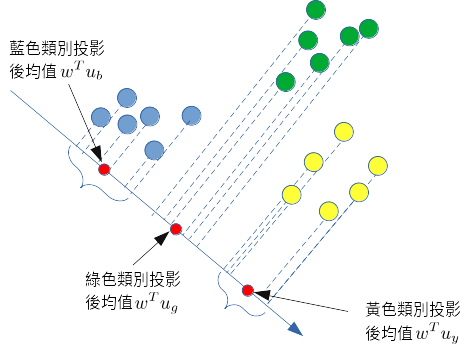
\includegraphics[height=5cm]{./pic/0JcYc52J.png}
		      \caption{部分資料經過投影的結果}
		      \label{fig:LdaTransform}
	      \end{figure}

	\item
	      根據前一小節提到的,希望投影過後「組內離散程度越小越好,組間離散程度越大越好」,最後會希望找到一個 \(w\),使得\(\frac{\mathbf{S_b}}{\mathbf{S_w}}\) 越大越好,如式(\ref{eqn:FindMaximun})。

	      \begin{equation}
		      \label{eqn:FindMaximun}
		      \underset{w}{max}\frac{\mathbf{{S_b}'}}{\mathbf{{S_w}'}} =\underset{w,w^TS_ww = 1}{max}\frac{\mathbf{{S_b}'}}{\mathbf{{S_w}'}}
	      \end{equation}


	      %
	\item
	      最後,圖\ref{fig:LdaDataLdaTransform}為此資料經過LDA轉換的結果,資料變得比較好區分。此外,圖\ref{fig:LdaDataPcaTransform}為經過PCA轉換的結果,雖然比原資料來的好,但是與LDA的結果相比,還是差了一些。
	      \begin{figure}[H]
		      \begin{center}
			      \begin{tabular}{ccccccccccccc}
				      \subfigure[資料經過LDA轉換的結果 ]{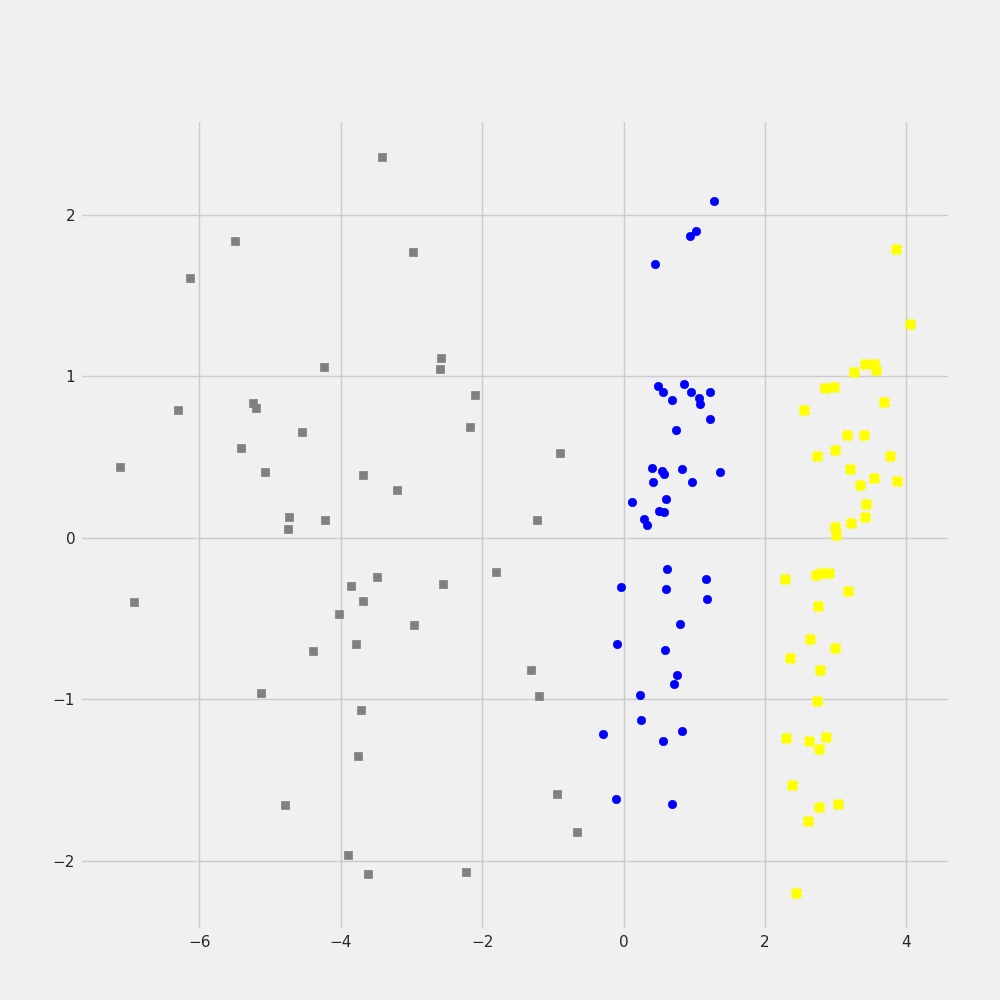
\includegraphics[width=7cm]{pic/lda_dataset_lda_transform.png}\label{fig:LdaDataLdaTransform} } \par &
				      \subfigure[資料經過PCA轉換的結果]{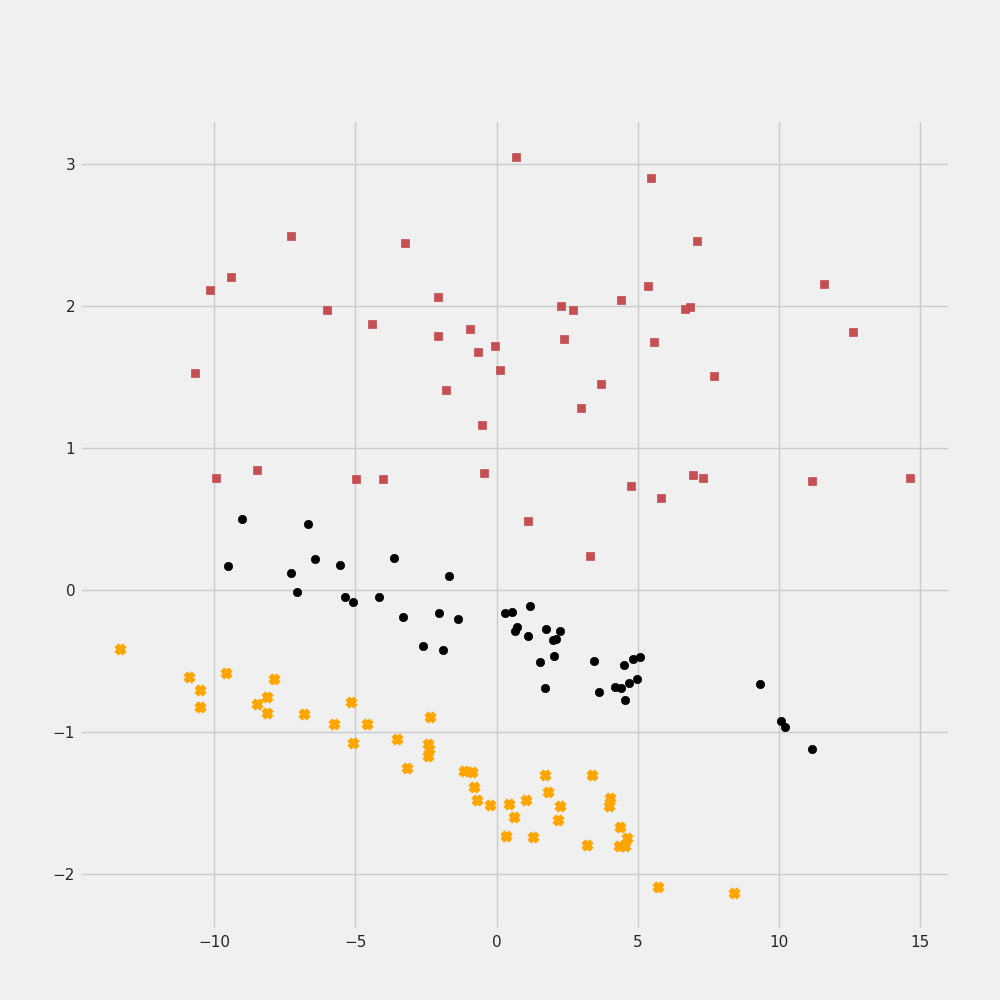
\includegraphics[width=7cm]{pic/lda_dataset_pca_transform.png}\label{fig:LdaDataPcaTransform} } \par    \\
			      \end{tabular}
			      \caption{資料集經過LDA與PCA轉換的結果}
			      \label{fig:LdaDataPcaLdaTransform}
		      \end{center}
	      \end{figure}


\end{itemize}


\section {結論}

從以上的實例中可以發現,因為LDA屬於監督式學習法,可以根據本生的類別,進行有效的降維,也因此相比之下,雖然運算時間較長,但能有比PCA有更好的效果。除此之外,也能發現經過LDA的分析後,我們僅需要一個維度就可以順利的將三個類別分離,可見LDA在進行降維處理,有著顯著的效果。


% MI	
\chapter{Mutual Information}
\label{chapter:intro}
\section{相互資訊(Mutual Information)}
它是衡量兩個隨機變量之間關係性存在和強度的指標。它通過查看另一個隨機變量來量化關於一個隨機變量中預期的“信息量”。也可以說假設有A和B兩事件,在B已發生的情況下,而A會發生所能提供的資訊。相互資訊不限於實值隨機變量和線性相關,並確定兩個變量之間的聯合分佈和邊際分佈的乘積的相似程度。
\begin{equation}
\label{equ:mi}
    \textbf{I}(X,Y)=\sum_{y\in Y}^{}\sum_{x\in X}^{}p(x,y)log(\frac{p(x,y)}{p(x),p(y)})
\end{equation}

        兩個屬性 X 和 Y 之間的相互信息,表示為 I(X, Y),它可以衡量對一個 屬性值的了解,能減少有關另一個屬性值的不確定性。如果 I(X, Y)很大,則可能存在一些相關性很強的連接在X和Y之間。





% Pearson	
\chapter{Pearson 相關係數}
\label{chapter:intro}
\section{Pearson 相關係數}
Pearson 相關係數時常在統計學中用於度量兩變量之間的線性相關程度, 該係數的值介於[−1,1],越接近 1 代表相關性越高,存在兩變量x=[x1,x2,……xi]和y=[y1,y2,……yi] ,其相關性$r_{xy}$定義為。

\begin{equation}
\label{eqn:Pearson }
    r_{xy}=\frac{t\ast \sum_{k=1}^{t}x_ky_k+\sum_{k=1}^{t}x_k\sum_{k=1}^{t}y_k}{\sqrt{t\ast \sum_{k=1}^{t}x_k^2-(\sum_{k=1}^{t}x_k)^2}\ast\sqrt{t\ast \sum_{k=1}^{t}y_k^2-(\sum_{k=1}^{t}y_k)^2}}
\end{equation}
其中rxy 範圍1跟-1之間,越靠近1正相關性越大,越靠近-1負相關性越大,越靠近零相關性越小。
    


% GA	
\chapter{Genetic Algorithm}
\label{chapter:intro}
\section{遺傳演算法(Genetic Algorithm, GA)介紹}
遺傳演算法是一種從遺傳科學中獲得啟發的技術,目前被廣泛應用於解決優化問題,尤其在特徵篩選方面。在GA中通常使用染色體的概念作為解決方案,通常基因數與特徵數相等,例如 \(Z=(0,1,1,0,1,0,0,0)\) 代表一染色體上共有8個特徵,1則代表以選擇特徵;0則代表未選擇特徵。
GA主要由三種運算組成,分別為親代選擇、交叉與突變。首先生成具有隨機染色體集合的初始群集,之後評估每個染色體的適合度,並從適合度的概率來選擇親代父母,接下來在親代父母之間進行交叉配對,生成從親代父母繼承基因的染色體特徵子集,此外根據突變率可能導致生成的染色體子集突變(即0變1或是1變0),之後評估新生成的染色體子集適合度,並將新生成的染色體子集加入當前的群集中,並根據適合度進行排序,選擇最佳的N條染色體應用於下一代,重複該算法直到設定的最大迭代次數為止,最後選擇全局最佳染色體作為最佳特徵子集。
\begin{figure}[H]
	\centerline{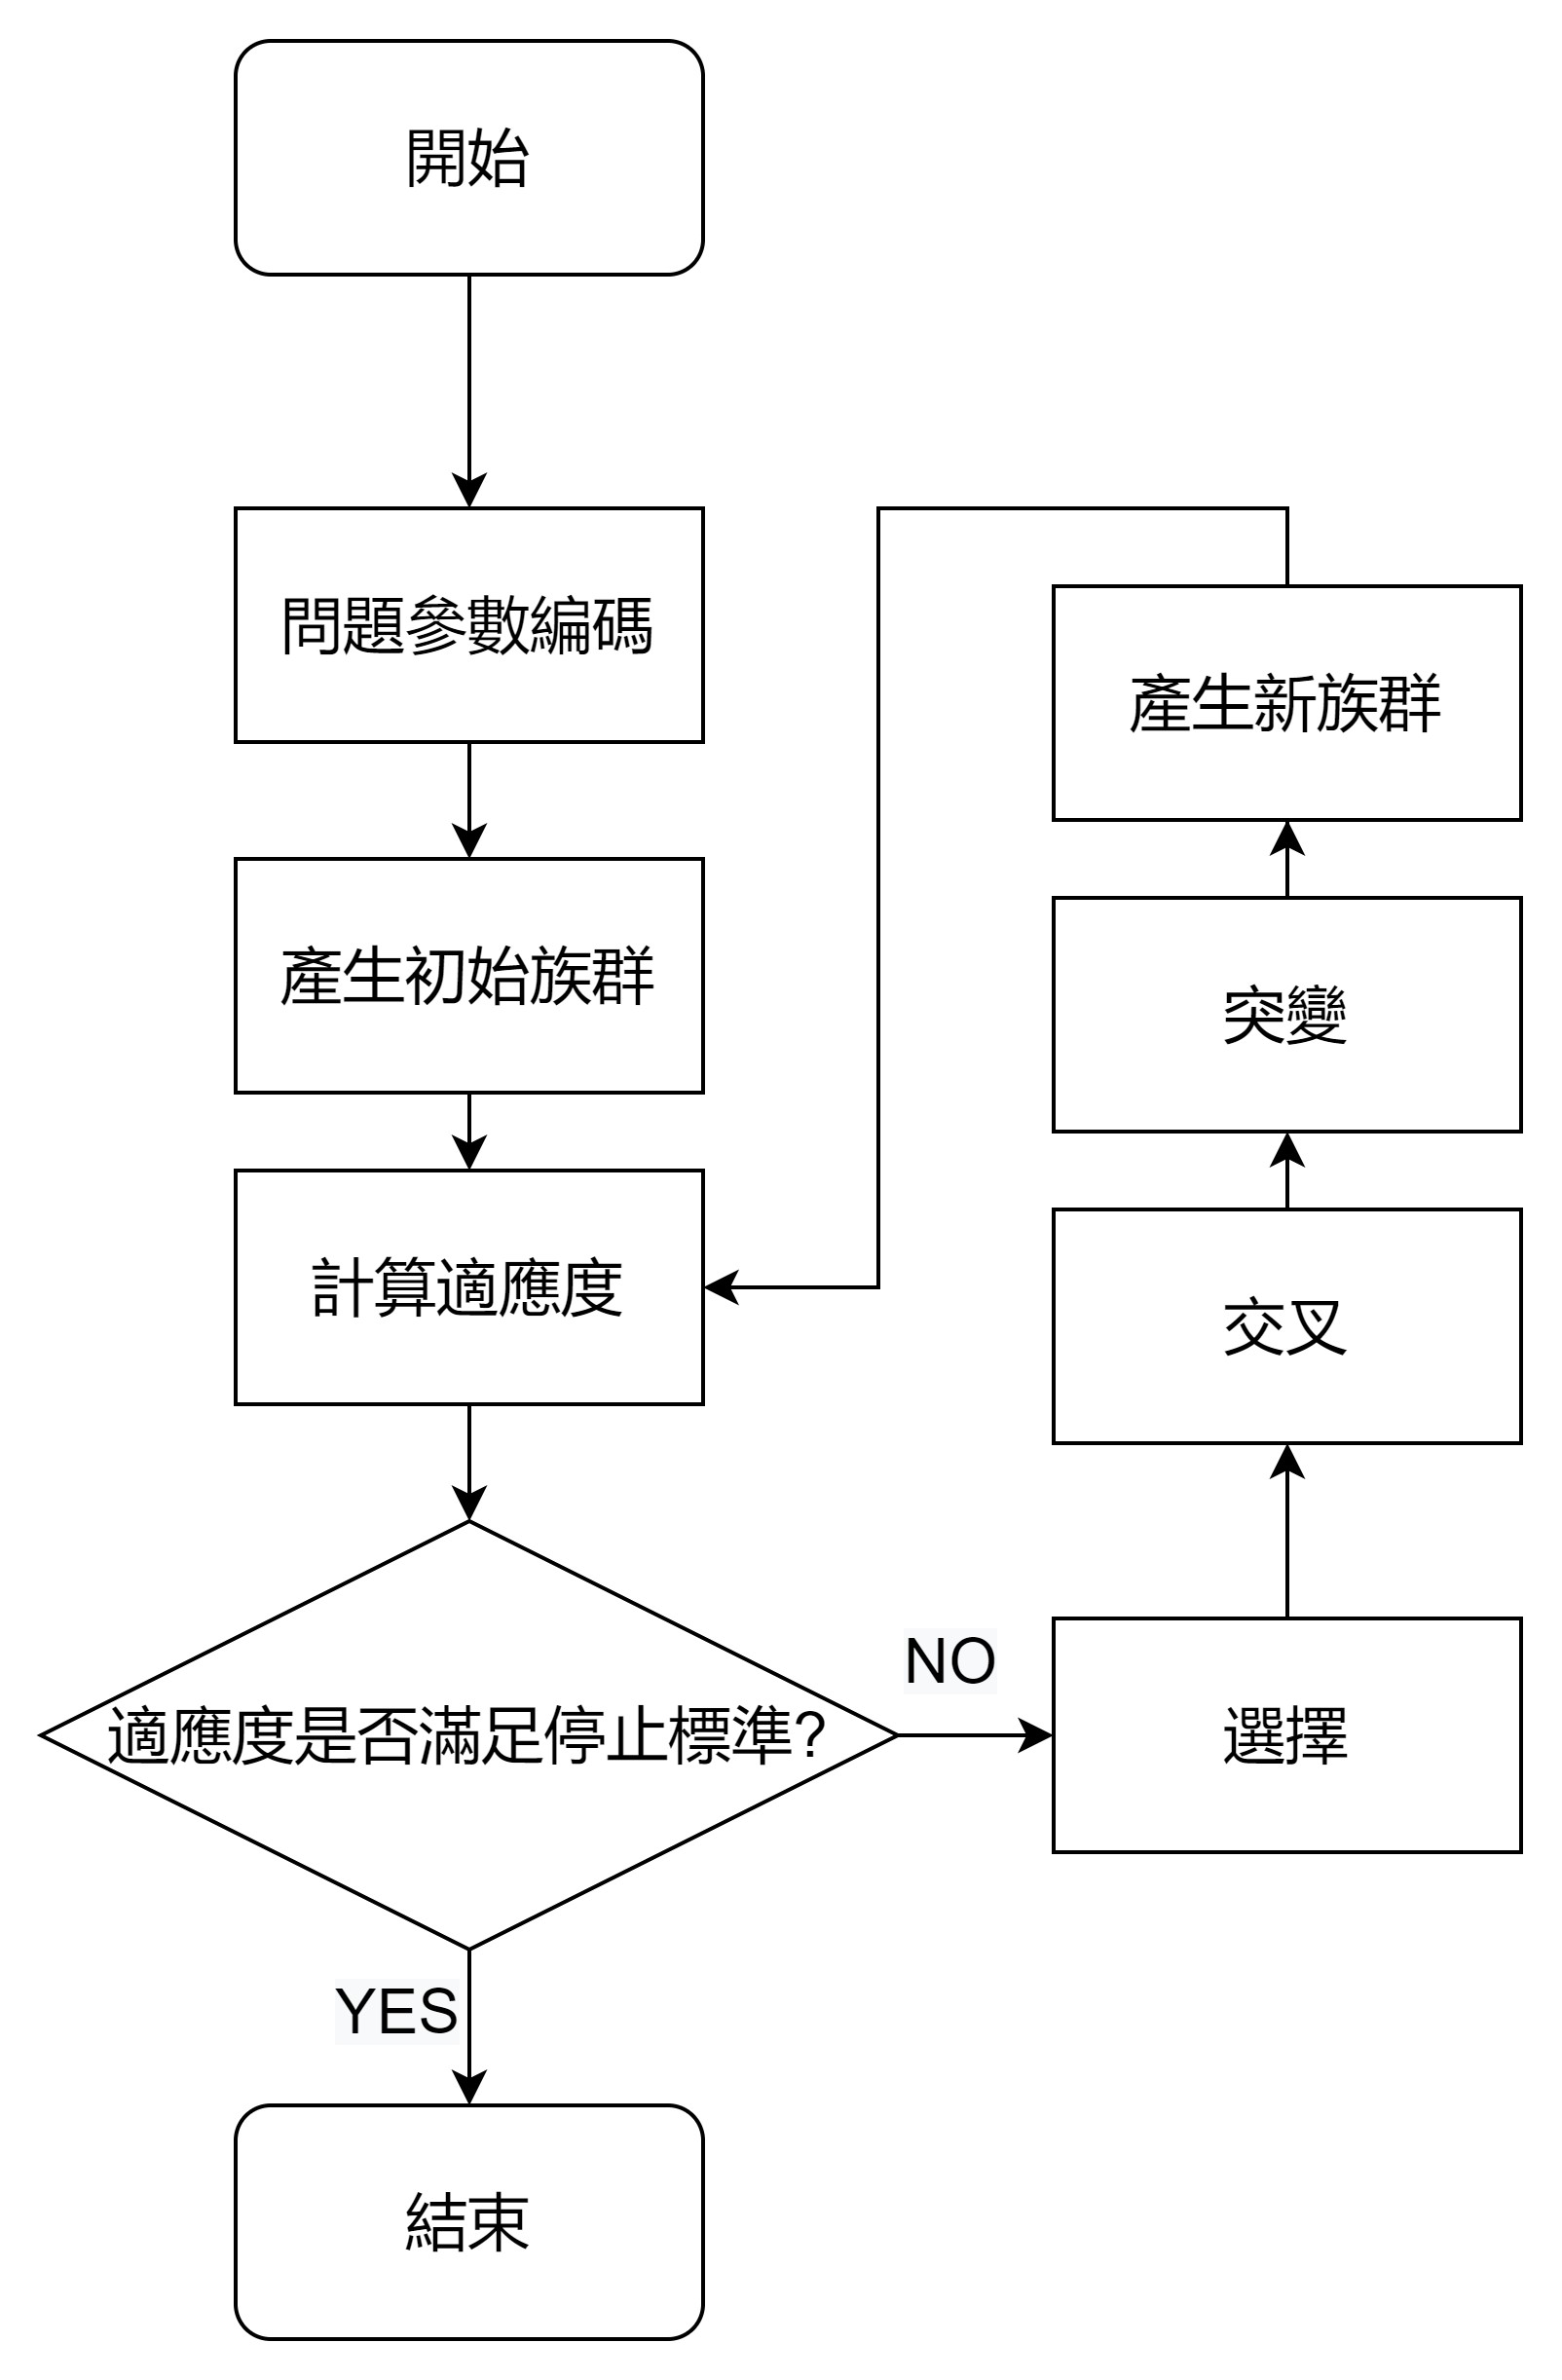
\includegraphics[height=8cm]{pic/GAFlowChart.PNG}}
	\caption{GA流程圖}
	\label{fig:GAFlowChart}
\end{figure}

\label{sec:background}
\section{問題參數編碼}
如何將一個問題所需處理的資料編碼 (Encode) 成染色體,
是GA的一個關鍵議題,染色體編碼是要利用GA來解決問題時的首要任務。其中最常見的是用二元編碼 (Binary Encoding) 。\\
二元編碼 (Binary Encoding),
將選好的特徵基因進行排序,1 則代表以特徵被選擇;0 則代表特徵未被選擇,假設一條染色體有五個特徵可以選擇,所構成的染色體從00000~11111共有32個可行解。

\section{適應度(Fitness)計算}

在每完成初始族群取選後,須針對所有被選取的個體,計算其適應能力,做為接下來選種的依據, 每一個個體都被評估後得到一個適應能力值,族群中的個體被按照適應度排序,適應度高的在前面,如果用代價函數(Cost Function)來當評估標準,則需看實際問題是要求最大值(Maximum)還是最小值(Minimum)。
\section{親代選擇}
GA使用選擇運算子來對群體中的個體進行優勝劣汰操作:根據適應函數評估出每一個個體的適應度值大小選擇,適應度較高的個體會被挑選 出來複製到下一代群體中的機率較大,適應度低的自然被選出來的機率就較小。 這樣可以使得群體中個體的適應度不斷的往最佳解的方向移動,而不是盲目搜尋。

\begin{enumerate}
	\item
	      輪盤式選擇(Roulette Wheel Selection):
	      首先要計算每一個體的適應度,然後計算出此適應度在群體適應度總和中所佔的比例,表示該個體在選擇過程中會被選中的機率,適應度越大被選擇的機率越大。選擇想法就是適應程度越好,所被選擇的機率越大,適應程度越差,被選擇的機率越小,如此以來,在選擇時適應程度越好的,也越有機會被選中,就如同生物進化過程中的「適者生存,不適者淘汰」的觀念,希望將優良基因會遺傳給下一代的個體。如果群體的適應度差異巨大時,最佳個體的被選擇機率會大幅成長,容易使這個最佳個體充斥在當前群體中,使得群體喪失多樣性,過早失去進化能力。
	      \begin{figure}[H]
		      \centerline{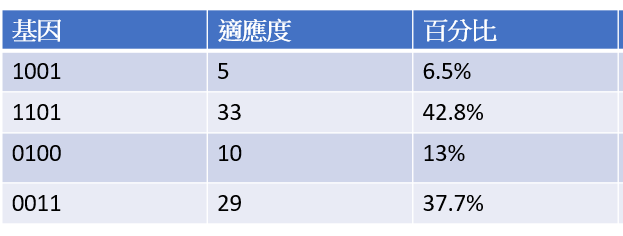
\includegraphics[width=10cm]{pic/Wheel.PNG}}
		      \caption{基因編碼與適應度}
		      \label{fig:GeneEncodeAndFitness}
	      \end{figure}
	      \begin{figure}[H]
		      \centerline{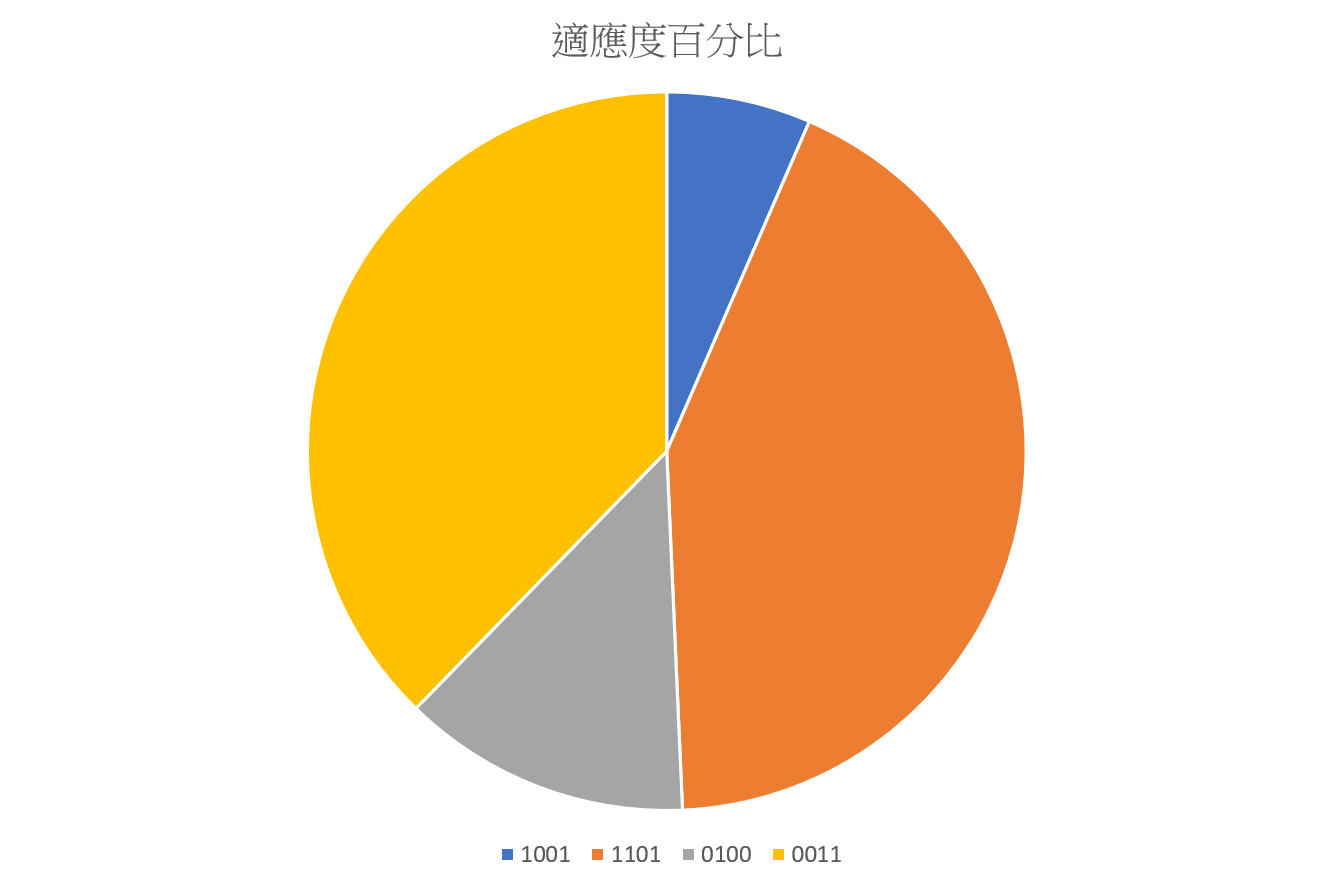
\includegraphics[width=10cm]{pic/wheelFitness.png}}
		      \caption{輪盤法適應度百分比圖}
		      \label{fig:WheelMethodPercentage}
	      \end{figure}
	      

	\item
	      競爭式選擇(Tournament Selection):
	      按照輪盤選擇的機率為依據,隨機取得幾個基因續列,並立即進行比較,將適應力較好的留下,因為是用機率選取基因,所以不但可以塞選出好基因,也能避免輪盤法則的缺點發生。
\end{enumerate}

\section{交叉(crossover)}
交叉將兩個父輩染色體上的基因進行重新組合分配,從而產生下一代個體的過程,通過交叉可能會將兩個父輩的優勢基因組合在一起,產生適應度更高、更接近最優解的新個體。

\begin{enumerate}
	\item
	      單點交叉:
	      單點交叉算法就是指定了單個交換點用於父輩的基因交換重組。如圖\ref{fig:SinglePointCross}
	      \begin{figure}[H]
		      \centerline{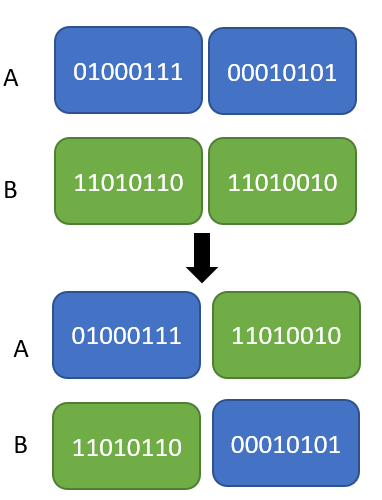
\includegraphics[height=6cm]{pic/one.PNG}}
		      \caption{單點交叉示意圖}
		      \label{fig:SinglePointCross}
	      \end{figure}

	\item
	      多點交叉:
	      多點交叉算法就是指定了多個交換點用於父輩的基因交換重組。如圖\ref{fig:MultiPointCross}
	      \begin{figure}[H]
		      \centerline{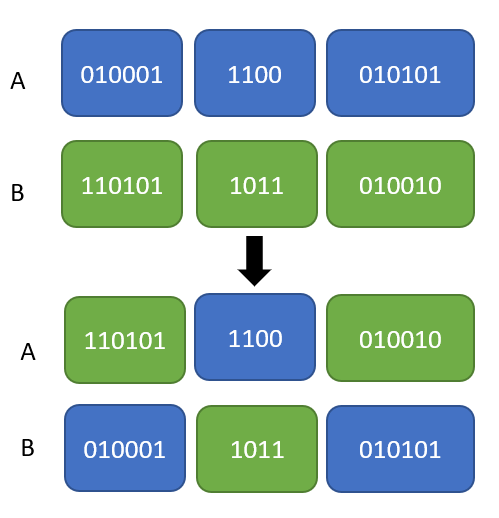
\includegraphics[height=6cm]{pic/TWO.PNG}}
		      \caption{多點交叉示意圖}
		      \label{fig:MultiPointCross}
	      \end{figure}

	\item
	      均勻交叉:
	      單點交叉跟多點交叉,存在染色體中某些部分的基因會被過早地捨棄,為了避免這個問題,有了均勻交叉,首先隨機選擇染色體上的交換位;然後隨機確定交換的基因是父輩染色體上交換位的前部分基因還是後部分基因;最後對父本染色體的基因進行重組從而產生新的下一代個體。如圖\ref{fig:avg}
	      \begin{enumerate}[(a)]
		      \item
		            隨機產生一個與個體長度相同的遮蔽字串W(Mask String)。

		      \item
		            若W=0則相對應父輩基因保留;若W=1則相對應父輩基因進行交叉。
	      \end{enumerate}
	      \begin{figure}[H]
		      \centerline{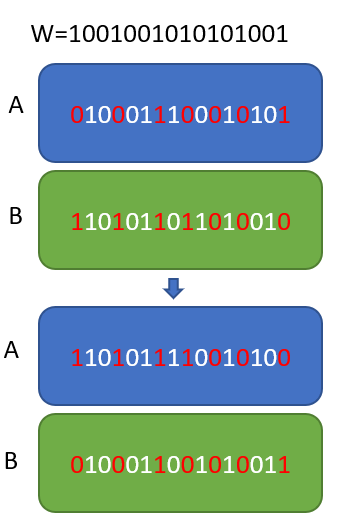
\includegraphics[height=6cm]{pic/AVG.PNG}}
		      \caption{均勻交叉示意圖W=1001001010101001}
		      \label{fig:avg}
	      \end{figure}


\end{enumerate}




\section{突變}
突變是為了避免種群中的染色體過於相似,使算法陷入區域極端,減慢或停止進化過程。遺傳算法利用交配操作從全局角度尋找一些較好的個體編碼結構,有助於獲得問題的最優解,但僅交配操作不能對搜索空間的細節進行局部搜索。這時,如果對個體編碼串中的一些基因值進行變異調整,個體可以從局部的角度更接近最優解,從而提高遺傳算法的局部搜索能力。突變示意圖\ref{fig:GAmut}

\begin{figure}[H]
	\centerline{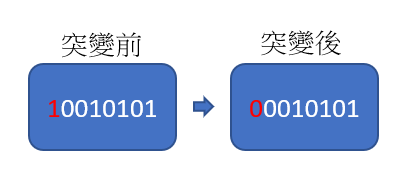
\includegraphics[height=2.5cm]{pic/GAmut.PNG}}
	\caption{突變示意圖}
	\label{fig:GAmut}
\end{figure}


%% CNN
\chapter{Convolutional Neural Networks}
\label{chapter:intro}
\section{CNN(Convolutional Neural Networks)介紹}
卷積神經網路(Convolutional Neural Network)為深度學習的分類模型,是一種前饋神經網路,對於大型圖像處理有出色表現,架構為一輸入層、數個隱藏層與一輸出層所組成,其中隱藏層包含有卷積層、池化層與全連接層。它與多層感知器不同點是並非所有神經元會全部連結。訓練過程是從訓練集中以梯度下降法來確定權重與偏差。
\begin{figure}[H]
	\centerline{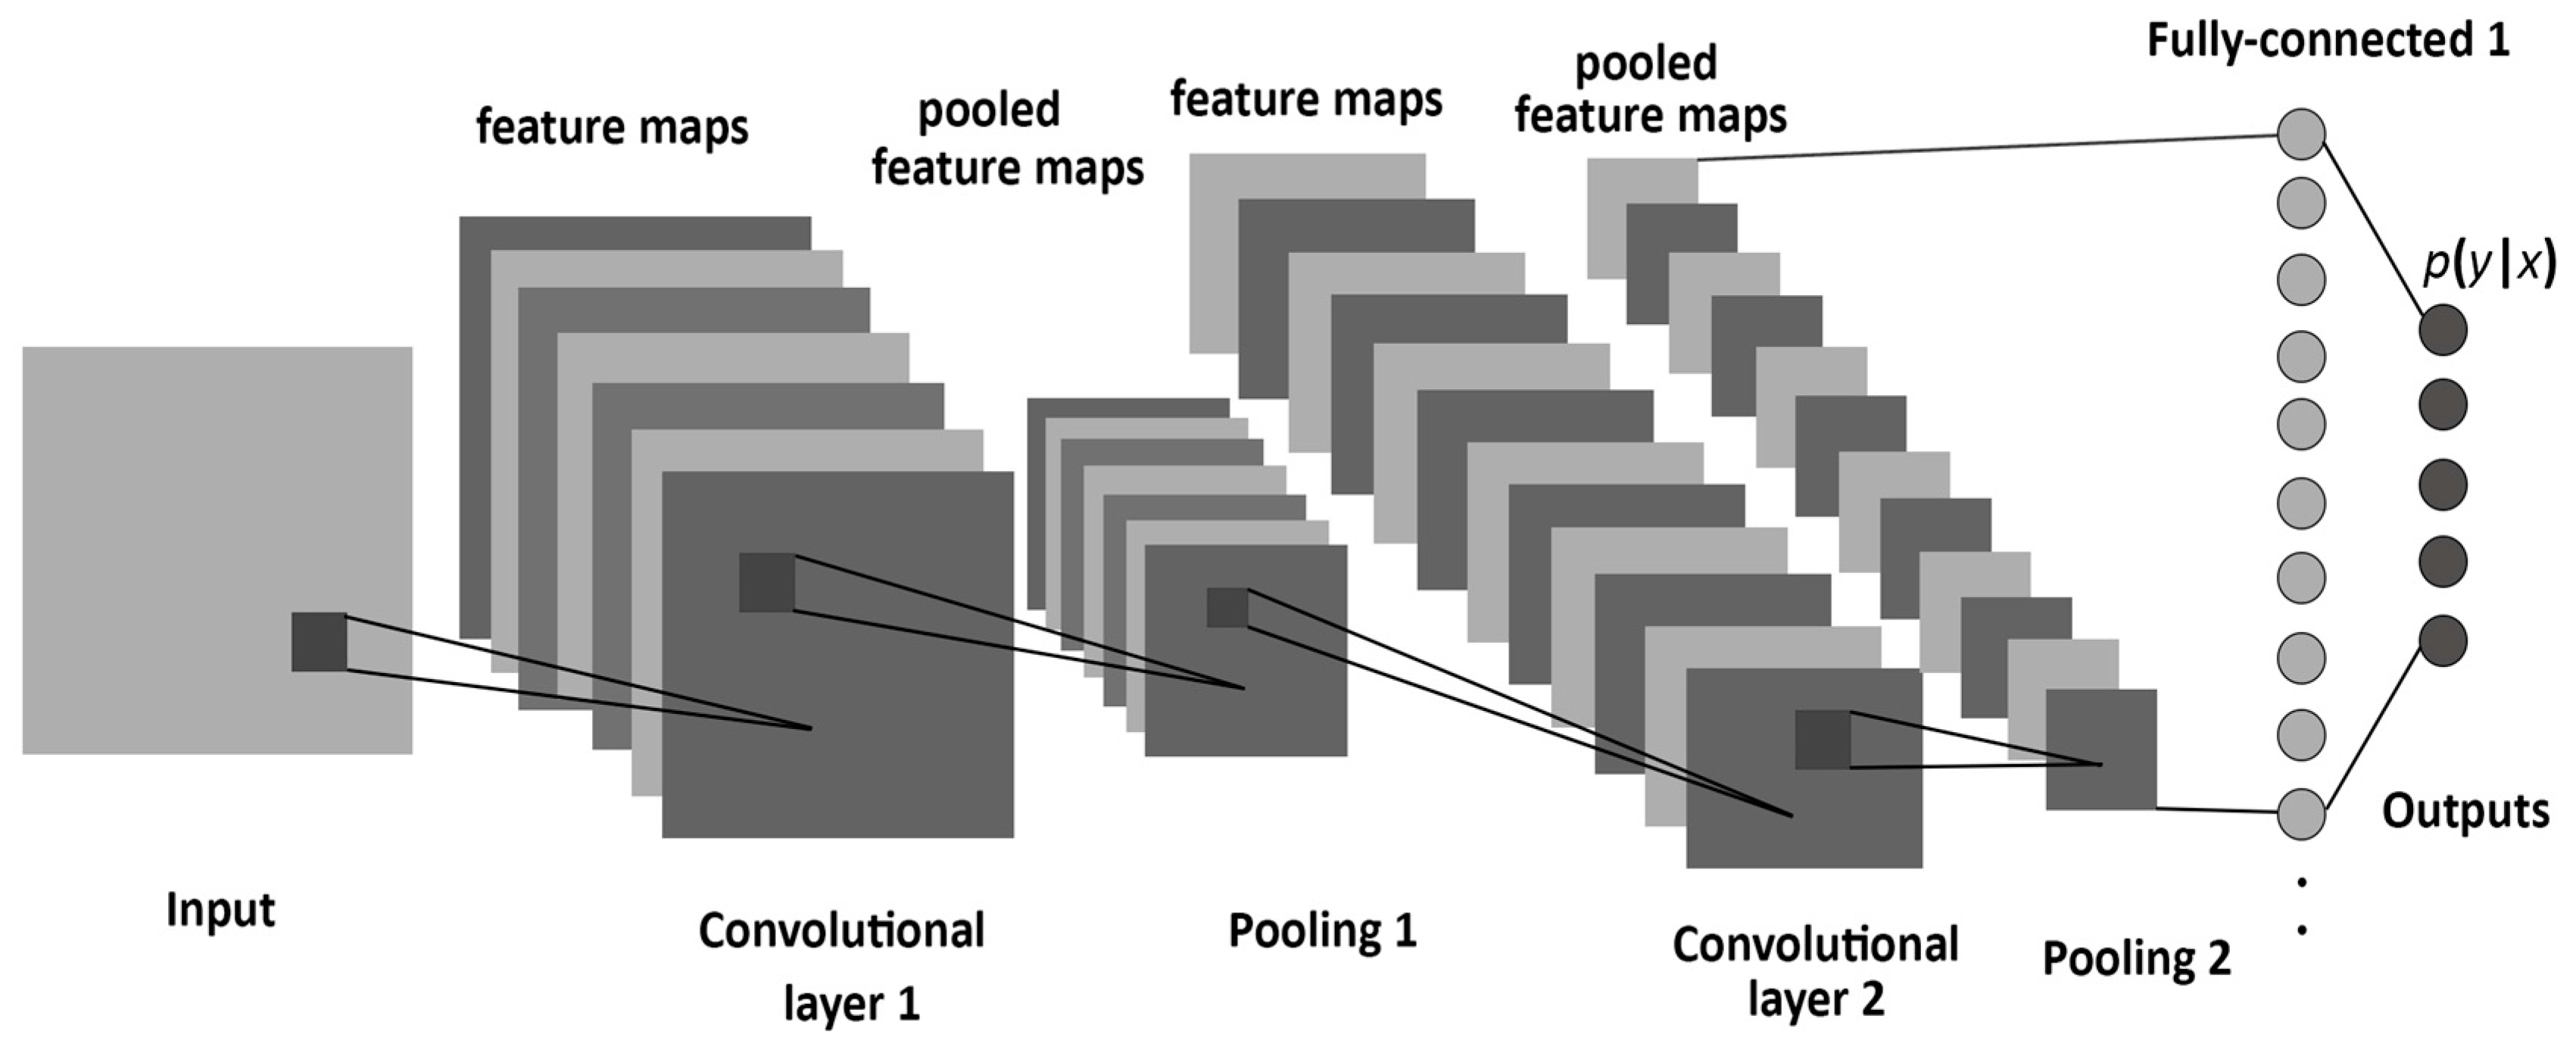
\includegraphics[height=7cm]{pic/CNNAR.png}}
	\caption{CNN架構圖}
	※引用:Saleh Albelwi and Ausif Mahmood(2017)。A Framework for Designing the Architectures of Deep Convolutional Neural Networks

	\label{fig:CNNAR}
\end{figure}


\label{sec:background}
\section{CNN(Convolutional Neural Networks)基本結構}
\subsection{輸入層(Input Layer)}
用於數據的輸入。
\subsection{卷積層(Convolution Layer)}

尋找特徵,CNN是根據影像的特徵來判別分類,不必由整個影像來判別。因為共用相同的特徵參數,如果對上不同影像,只要有相同的特徵出現,就算在不同的區域依然可以找到。

尋找特徵方法:
使用遮罩(Mask)在原始影像上移動,濾波器的值對遮罩內的值作內積計算,這過程稱為卷積(Convolution)。


輸出第一格數據為2x(-1)+2x0+0x0+0x0+1x0+1x0+0x1+1x0+2x1+1x1=1,以此類推一次往右一格到邊界時,往下一列從新從第一行開始,計算得出,計算得出卷積(Convolution)結果。


\begin{figure}[H]
	\centerline{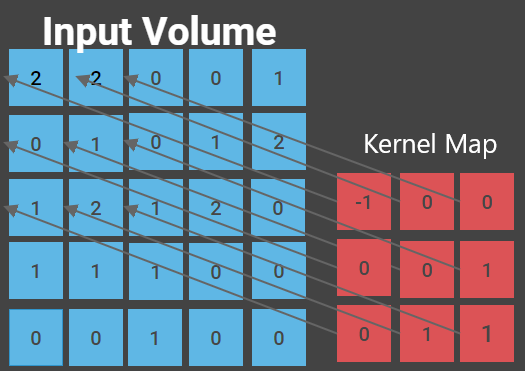
\includegraphics[height=7cm]{pic/CNN1.png}}
	\caption{卷積(Convolution)示意圖}
	\label{fig:CNN}

	\centerline{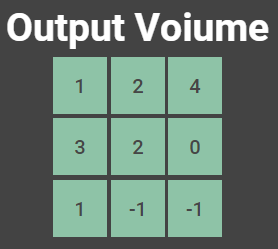
\includegraphics[height=5cm]{pic/CNN2.PNG}}
	\caption{卷積(Convolution)結果示意圖}
	\label{fig:CNN finally}
\end{figure}



具有特徵的濾波器內的權重其數值取得,一開始設置初始權重,因為一開始特徵並不是最好的特徵,因此模型預測與標籤所計算的誤差會非常高。但透過梯度下降法更新濾波器的權重,隨著訓練多次迭代,它會自動趨近於它認為最好的特徵,這特點稱為自動提取特徵。

卷積前後影像大小改變:

是否進填充將影響影像大小的改變,上述例子是採用VALID padding圖\ref{fig:CNN},不在原有的影象基礎上做任何填充,但這樣會有個缺點,在卷積多次後,可能使邊緣的畫素和卷積核做卷積的次數小於影象中間的畫素點,從而導致對其資訊的特徵的提取不足。

所以另一個方法SAME padding,使得做卷積運算後,原始影象的大小會保持原樣。
填充的大小計算公式:
\begin{equation}
	\label{equ:padding}
	P=(F-1)/2
\end{equation}
\\

P為填充\\
F為卷積核的寬 ( 高 ) 度
\begin{figure}[H]
	\centerline{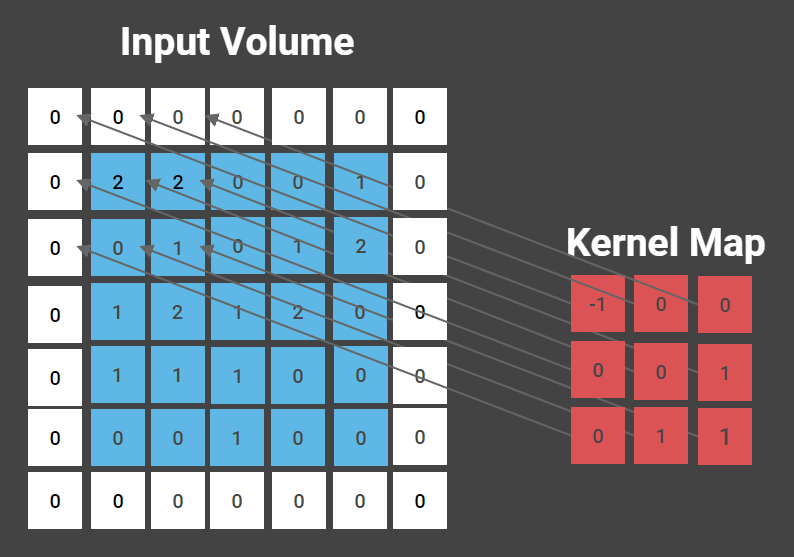
\includegraphics[height=7cm]{pic/samepadding.PNG}}
	\caption{卷積(Convolution)有填充示意圖}
	\label{fig:samepadding}
\end{figure}
\begin{figure}[H]
	\centerline{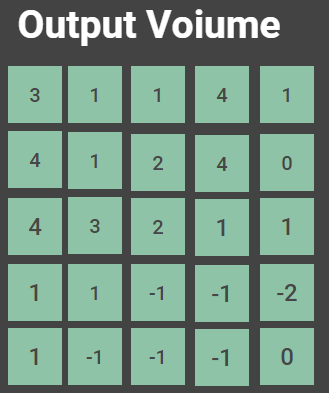
\includegraphics[height=5cm]{pic/samepaddingout.PNG}}
	\caption{卷積(Convolution)有填充結果示意圖}
	\label{fig:samepaddingout}
\end{figure}


卷積前後影像大小計算:
\begin{equation}
	\label{equ:mi}
	Woutput=(Winput-F+2P)/S+1
\end{equation}

\begin{enumerate}
	\item
	      Woutput為特徵圖的寬 ( 高 ) 度
	\item
	      Winput為前圖像寬 ( 高 ) 度
	\item
	      F為卷積核的寬 ( 高 ) 度
	\item
	      P為填充,使用填充:原始影像周圍補上零
	\item
	      S為步長(每次移動遮罩的距離)
\end{enumerate}
圖\ref{fig:CNN}是5X5的影像經過3X3濾波器每次一步,不進行填充,計算卷積後影像大小:\\
(5-3+2*0)/1+1=3,卷積後影像大小為3X3\\
圖\ref{fig:samepadding}是5X5的影像經過3X3濾波器每次一步,進行填充,計算卷積後影像大小:\\
(5-3+2*1)/1+1=5,卷積後影像大小為5X5




\subsection{池化層(pooling Layer)}
對影像進行欠取樣(Undersampling)使影像大小在不改變特徵時減少像素,達到減少運算時的數據量。
上述方法稱為:池化,池化是先在圖片上選取不同窗口(window),並在這個窗口範圍中依據不同方法選擇一個特徵值。
如果是使用2X2的窗口,原圖經過池化以後,其所包含的像素數量會降為原本的四分之一,如\ref{fig:Pooling Layer}圖6X6的圖檔經過2X2的窗口進行池化,變成3X3的特徵圖
但因為池化後的圖片包含了原圖中各個範圍的特徵值,保留了每個範圍內各個特徵的相符程度。池化後的資訊更專注於圖片中是否存在相符的特徵,而非圖片中哪裡存在這些特徵。這能幫助 CNN 判斷圖片中是否包含某項特徵,而不必分心於特徵的位置。\\
◼ 局部最大池化(Max Pooling)\\
取所有元素的最大值。\\
如圖\ref{fig:Pooling Layer}第一個窗口數字為[0.8,0.7,1,0.5] 局部最大池化選取所有元素的最大值,此窗口最大值為1,選擇1為特徵值。\\
◼ 局部平均池化(Average Pooling)\\
取所有元素的平均值。\\
如圖\ref{fig:Pooling Layer}第一個窗口數字為[0.8,0.7,1,0.5] 局部平均池化選取所有元素的平均值,所以(0.8+0.7+1+0.5)/4=0.75,所以選擇0.75為特徵值。\\
\begin{figure}[H]
	\centerline{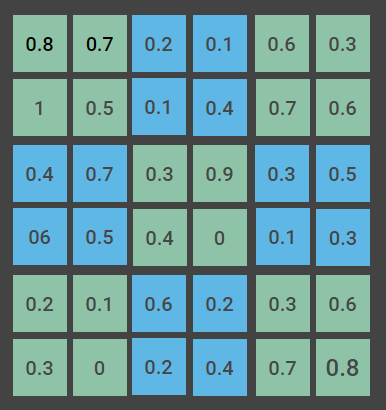
\includegraphics[height=10cm]{pic/pooling 1.PNG}}

	\caption{Pooling Layer示意圖}
	\label{fig:Pooling Layer}
\end{figure}
\begin{figure}[H]
	\centerline{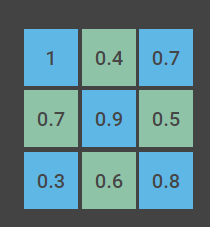
\includegraphics[height=5cm]{pic/poolinig 2.PNG}}
	\caption{Max Pooling示意圖}
	\label{fig:Max Pooling}
\end{figure}
\begin{figure}[H]
	\centerline{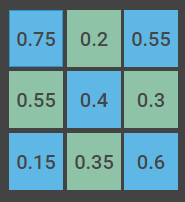
\includegraphics[height=5cm]{pic/pooling 3.PNG}}
	\caption{Average Pooling示意圖}
	\label{fig:Average Pooling}
\end{figure}


\subsection{全連接層(Fully Connected Layer)}
將所有特徵圖變為一維度,並組合在一起來進行輸出分類,簡單的來說就是一個分類器,把我們經過數個卷積、池化後的結果進行分類。
把我們經過數個卷積、池化後的結果進行分類。通 常 在 全 連 接 層 與 輸 出 層 間 會 使 用 Softmax(歸一化指數函式)函數來輸出機率,使所有類別的機率和為1。
\subsection{輸出層(Output Layer)}
用於最後輸出結果。


\section{CNN(Convolutional Neural Networks)訓練過程與參數設定}
\subsection{演算法參數}
model.add=(Convolution2D(output size,Kernal Size,padding方法,input shape =(img channels,img rows,img cols))
model.add(激活函數)
\begin{enumerate}
	\item
	      輸入圖片:img channels:圖片類別,img rows,img cols:圖片的寬高
	\item
	      設定卷積核大小Kernal Size(6,6)
	\item
	      output size:卷積後的深度
	\item
	      padding方法:有VALID padding和SAME padding
	\item
	      激活函數使用ReLU函數,式\ref{equ:REIU}
	      \begin{equation}
		      \label{equ:REIU}
			  Relu(x)= 
\left\{\begin{matrix}
x \ \ \ \ \ \ if\ x>0
\\ 
0 \ \ \ \ \ \ if\ x<0
\end{matrix}\right.
	      \end{equation}
\end{enumerate}
CNN演算法如圖\ref{fig:keras}所示
\begin{figure}[H]
	\centerline{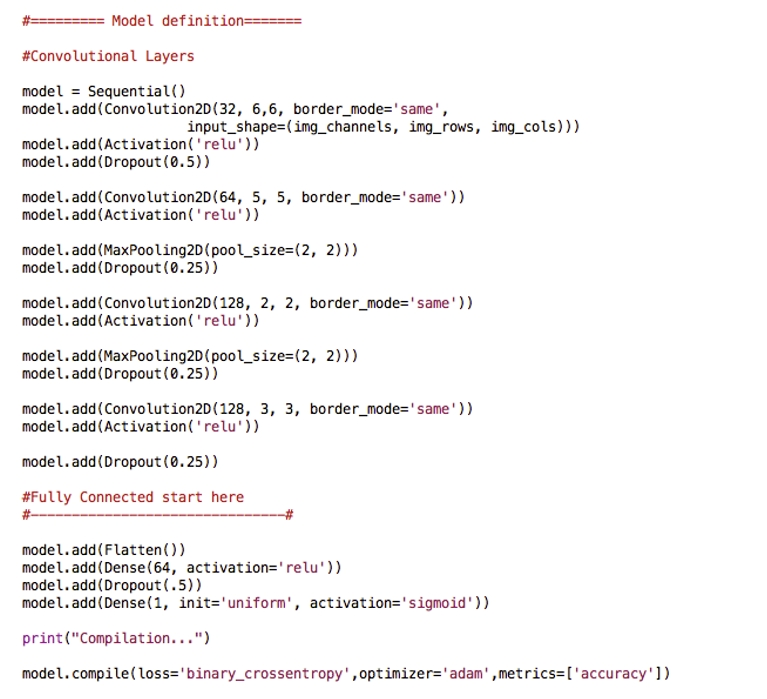
\includegraphics[height=15cm]{pic/Keras.jpg}}
	\caption{CNN演算法圖}
	\label{fig:keras}
\end{figure}

\subsection{CNN(Convolutional Neural Networks)訓練過程}
\begin{enumerate}
	\item
	      初始化網絡權重。
	\item
	      輸入數據經過卷積層、池化層、全連接層的向前傳播得到輸出值。
	\item
	      求出網絡的輸出值與目標值之間的誤差,判斷是否達到設定的訓練目標。
	\item
	      並將誤差傳回網絡中,反向求得全連接層,池化層,卷積層的誤差。
	\item
	      根據求得誤差進行權重更新,用更新的權重進行回到第二步。
\end{enumerate}
\begin{figure}[H]
	\centerline{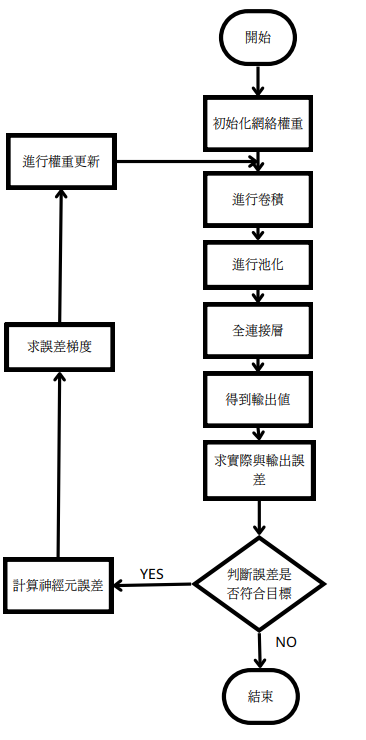
\includegraphics[height=15cm]{pic/CNNp.PNG}}
	\caption{CNN訓練流程圖}
	\label{fig:this_system}
\end{figure}
\section{CNN(Convolutional Neural Networks) 結語}
卷積神經網路,因為可以進行局部權重共享的特殊性質,在圖形辨識方面有著獨特的優勢,權重共享降低了網路的複雜性,特別是在處理多維輸入的向量圖像,只要有鄰近資料相關性,三維或多維度的資料也都可以使用。


%%  LVQ
\chapter{Learning Vector Quantization Neural Network}
\label{chapter:lvq}
\section{簡介}

%%圖\ref{fig:lvq_network}爲LVQ的網路架構圖。SOM是一個分群的演算法,如果將它的概念轉成監督式學習,就是LVQ演算法的由來。這個演算法可用於分類的應用,且具有簡單的架構。

學習向量量化(Learning Vector Quantization,簡稱爲LVQ),可以將其視爲是一種人工神經網路的特例。
圖\ref{fig:lvq_network}爲LVQ的網路架構圖。
從圖中可以發現這個網路僅具有輸入與輸出兩層,所以是一個結構相當簡單的神經網路,並且是一個具有監督式學習的分類演算法。
此外,在這個演算法中,採取了非監督式學習的機制,應用於監督式學習的問題上。


\begin{figure}[h]
	\centering
	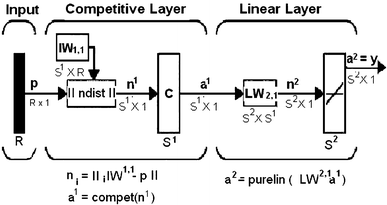
\includegraphics[width=10cm]{./pic/lvq_struct.png}
	\caption{LVQ網路架構圖}
	\begin{minipage}{.7\linewidth}
		\footnotesize
		\emph{圖片來源:}取自Seafloor sediment classification from single beam echo sounder data using LVQ network
	\end{minipage}
	\label{fig:lvq_network}
\end{figure}
\label{sec:background}


\section{Vector Quantization}
在理解LVQ演算法前,我們先來看看Vector Quatization。這個算法的目的主要是將原資料分割k個域區,並在這些分割的區域中,找出一個最能代表整個群組的向量,作為這個區域中的代表點。
這些代表點的集合我們稱爲codebook。
此外這個算法所做的事情有點類似將資料進行分群。
LVQ就是基於這個演算法的概念進行,透過監督式學習,不斷的更新代表的位置,進而找出最佳的codebook。


從圖\ref{fig:data_after_vq},可以看到原資料被分割成3個區域,以及3個紅色方點,而紅色方點就是整個分割區域中的代表點,也是LVQ中的weight vetcor。


\begin{figure}[h]
	\begin{center}
		\begin{tabular}{ccccccccccccc}
			\subfigure[原資料集分佈]{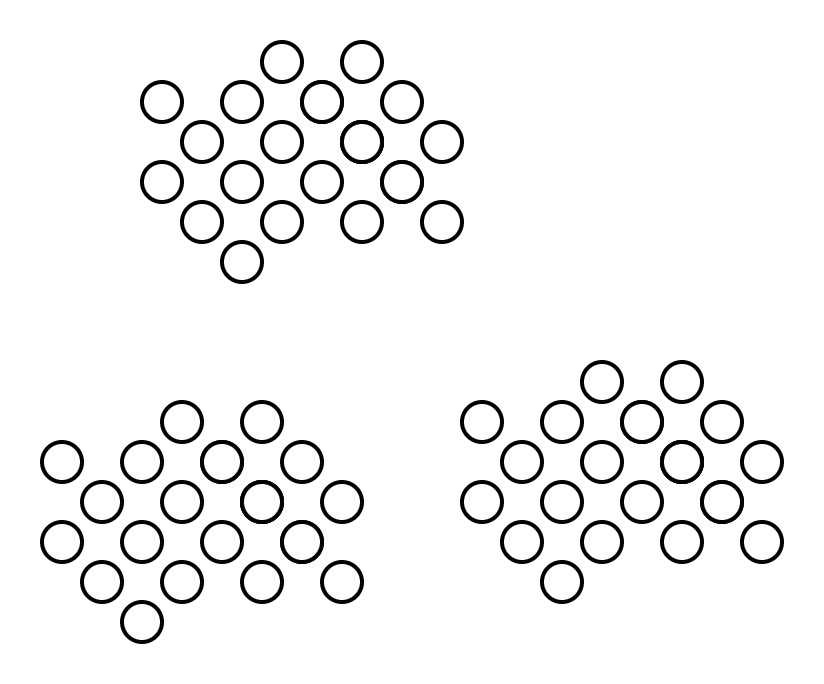
\includegraphics[height=4cm]{./pic/oA5nFv7C.png}\label{fig:ori_data} } \par &
			\subfigure[經過向量量化的原資料]{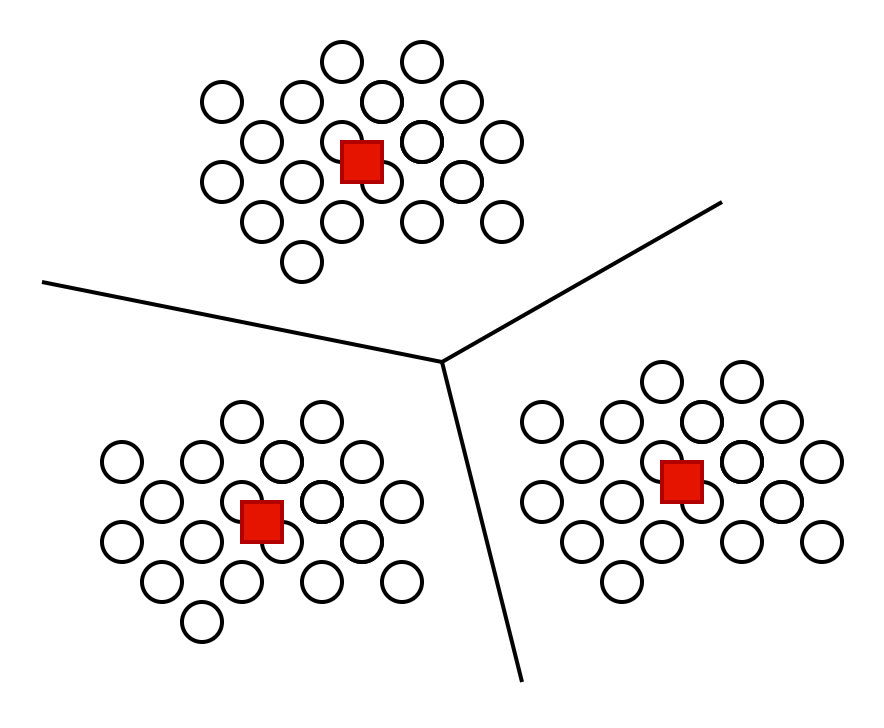
\includegraphics[height=4cm]{./pic/aLVdIIWU.png}\label{fig:data_after_vq} } \par \\
		\end{tabular}
		\caption{向量量化的示意圖}
		\label{fig:vector_quantization}
	\end{center}
\end{figure}



%%- 權重向量爲,$$\mathbf{w_{j}} = (w_{1j},w_{2j},w_{3j},....,w_{nj})$$
%%- 距離的計算採用,尤拉距離公式 $$D(j)=||\mathbf{x}-\mathbf{w_j}||_2 = \sqrt{(x_1-w_{1j})^2+(x_2-w_{2j})^2+...+(x_n-w_{nj})^2} $$
%%- $$C_j$$ 為網路層的輸出類別。
%%- $$T$$ 為每筆資料所對應的實際類別。
%%- $$\alpha$$爲學習率


\section{演算法參數定義與流程}

%%在這個演算法中只有Input Layer與Output Layer

\subsection{參數定義}

\begin{itemize}
	\item
	      輸入向量,\(\mathbf{x} = (x_1,x_2,x_3,....,x_R)\),爲資料集中的其中一筆資料,輸入向量的數量 \(d\) 爲資料的特徵數量。


	      %
	\item
	      競爭層權重,\(\mathbf{W^1} = (\mathbf{w_1,w_2,...,w_j,...w_R})^T\),爲一個 \(S^1 \times R \)的矩陣,也就是剛剛介紹Vector Quantization所提到的codebook,這邊的 \(n\)爲輸出的類別數量。
	      %
	\item
		權重向量,\(\mathbf{w_{j}} = (w_{1j},w_{2j},w_{3j},....,w_{dj})^T\),代表每個區域的代表點。

	      %
	\item
	      \(D(j)\)爲每筆資料與代表點的距離。
	      $$D(j)=||\mathbf{x}-\mathbf{w_j}||_2 = \sqrt{(x_1-w_{1j})^2+(x_2-w_{2j})^2+...+(x_n-w_{nj})^2} $$


	\item
	      %\(C_j\) 為網路層的輸出類別。
		\(\mathbf{C}\) 為競爭層的輸出向量。

	\item
	      輸出層權重,\(\mathbf{W^2} \)為一個 \(S^2 \times S^1\)的矩陣。

	\item
		\(\mathbf{y}\) 為網路的輸出向量。

	\item
	      \(\alpha\) 爲學習率
	\item
		此外,這裡為了方便說明,將 \(\mathbf{W^2}\) 設定為一個 \(S^1 \times S^1\) 的單位矩陣,也因此競爭層的輸出為網路層的輸出 \(\mathbf{C} = \mathbf{y}\)。

\end{itemize}


\subsection{流程}

首先會先初始化 \(\mathbf{W^1},\alpha\),接著將所有的訓練資料集中的每一筆資料,找出與每筆資料最近權重向量,並接著判斷 \(\mathbf{y}\) 的結果是否符合這筆資料的類別,如果相同就使得這個權重向量靠近這筆資料點且更新學習率,反之,如果不同則遠離。接著不斷重複以上步驟,直到訓練次數或是學習率達到設定的標準,則停止模型訓練。下圖爲演算法的流程圖\ref{fig:alogrithm_workflow}。

\newpage

\usetikzlibrary{positioning, shapes.geometric}

\tikzset{every picture/.style={line width=1.75pt}}


\begin{figure}
	\centering
	
	\resizebox{300pt}{400pt}{
		\begin{tikzpicture}[scale=1]
			\node[draw, rounded corners,align=center ]                        (start)   {初始化參數 \(\mathbf{W},\alpha\) };
			\node[draw,diamond, below=20pt of start,align = center]                        (step 2)  {訓練 \(\mathbf{x}\) 中的\\每一筆資料};
			\node[draw,  aspect=2, below=20pt of step 2]     (step 3)  {找出 \(min\{D(1),D(2),...,D(j),..D(d)\}\) };
			\node[draw, diamond,below=20pt of step 3]                   (compare)  {比對 \(y\)與 \(T\)  };
			\node[draw, below =30pt of compare,align = center]                         (same)  {\(\mathbf{w_j(new)} = \mathbf{w_j(old)} + \alpha(\mathbf{x} - \mathbf{w_j(old)})\)  };
			\node[draw, below right=55pt and 80pt of compare]                         (different)  {\(\mathbf{w_j(new)} = \mathbf{w_j(old)} - \alpha(\mathbf{x} - \mathbf{w_j(old)})\)};
			\node[draw, rounded corners, below=20pt of same]  (learning_rate)     {更新學習率 \(\alpha\) };
			\node[draw,diamond, below=20pt of learning_rate,align = center]                         (end_detect)  {判斷是否\\達到結束條件};
			\node[draw, rounded corners, below=20pt of end_detect]  (end)     {End};

			\draw[->] (start)  --coordinate(le) (step 2);
			\draw[->] (step 2) --node[left]{Yes} (step 3);
			\draw[->] (step 2.west) --node[above]{Yes}++(-50pt,0)|-(end_detect.west);
			\draw[->] (step 3) -- (compare);
			\draw[->] (compare) -> node[left]{Yes}(same.north);
			\draw[->] (compare.east) --node[above]{No}(compare.east-|different.north) -> (different.north);
			\draw[->] (same) -- (learning_rate);
			\draw[->] (learning_rate) -> (end_detect);
			\draw[->] (end_detect) -- node[left]{Yes}(end);
			\draw[->] (end_detect.east) --node[above]{No}++(250pt,0pt)|-(le) ;

		\end{tikzpicture}
	}

	\caption{演算法流程圖}
	\label{fig:alogrithm_workflow}
\end{figure}



%要被單行註解的文字。

\begin{comment}
要被區塊註解的文字,要被區塊註解的文字,要被區塊註解的文字,
要被區塊註解的文字,要被區塊註解的文字,要被區塊註解的文字,
要被區塊註解的文字,要被區塊註解的文字,要被區塊註解的文字,
要被區塊註解的文字,要被區塊註解的文字,要被區塊註解的文字,
要被區塊註解的文字,要被區塊註解的文字,要被區塊註解的文字,
要被區塊註解的文字,要被區塊註解的文字。
\end{comment}

\section{實例說明}

爲了能夠更簡單理解這個演算法的目的與實際的效果,以下以簡單的實例說明。
表\ref{tab:lvq_table}爲此次實例的資料集,此資料集分別有x跟y兩個特徵,以及兩種類別,並分別以綠色與紅色表示。


\begin{table}[h!]
	\centering
	\caption{資料集}
	\label{tab:lvq_table}
	\begin{tabular}{rrrr}
\toprule
  & x & y & Class  \\
\midrule
 & 1  & 3  & 1     \\
 j 6  & 1  & 2     \\
 & 3  & 4  & 1      \\
 & 8  & 3  & 2     \\
 & 9  & 1  & 2     \\
 & 1  & 6  & 1 	\\     
\bottomrule
\end{tabular}

\end{table}


\begin{figure}[h!]
	\centering
	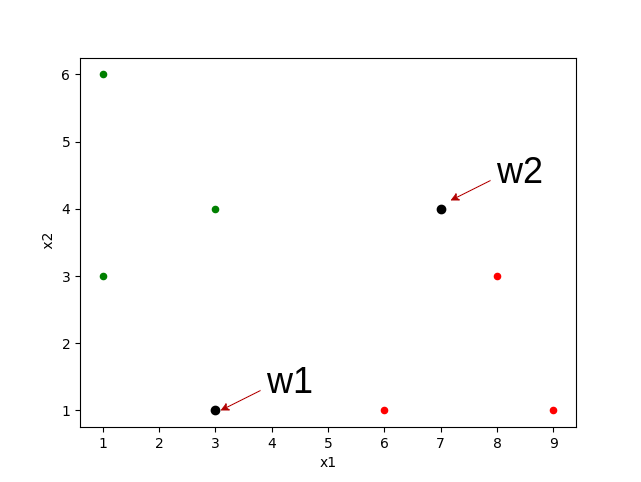
\includegraphics[height=10cm]{./pic/2nSRVeud.png}
	\caption{資料集在座標軸的分佈}
	\label{fig:dataset_in_axis}
\end{figure}

\newpage
\begin{enumerate}
	\item
	      首先先初始化 \(\mathbf{W}\),因爲這次的範例中只有兩個類別,這邊以 \(\mathbf{w_1}=(3,1),\mathbf{w_2}=(7,4)\)作爲初始化的兩個weight vector。並將學習率 \(\alpha\)的初始值設爲0.5,以及iteration設定爲100。
	      圖 \ref{fig:dataset_in_axis}爲此資料集與初始兩個weitght在座標軸的分佈。
	      %
	\item
	      接著計算第一筆資料與兩個weight vector的歐式距離,並比較兩個距離的大小。

	      $$D(1)=||\mathbf{x}-\mathbf{w_1}||_2 = \sqrt{(1-3)^2+(3-1)^2}=\sqrt{8}=2.8284 $$
	      $$D(2)=||\mathbf{x}-\mathbf{w_2}||_2 = \sqrt{(1-7)^2+(3-4)^2}=\sqrt{37}=6.0827 $$
	      $$D(1)<D(2)$$

	      %
	\item
	      由上一步得知 \(D(1)<D(2)\),所以此筆資料的神經網路的輸出結果 \(C_1\) 爲1,又因爲 \(C_1 = T = 1\),所以更新 \(\mathbf{w_1}\)要往 \(x\)的方向前進。此外,也因爲輸出結果與實際類別相同所以還要更新學習率的值。
	      $$\mathbf{w_1}(new) = \mathbf{w_1}(old) + \alpha(\mathbf{x-w_1}(old))= \begin{bmatrix}3\\ 1\end{bmatrix}+0.5(\begin{bmatrix}1\\ 3\end{bmatrix} - \begin{bmatrix}3\\ 1\end{bmatrix})= \begin{bmatrix}2\\ 2\end{bmatrix}  $$
	      $$\alpha(new) = \alpha(old)\times \frac{1}{1+decay*iteration} =0.4950$$

	\item
	      接著換第二筆資料
	      $$D(1)=||\mathbf{x}-\mathbf{w_1}||_2 = \sqrt{(6-2)^2+(1-2)^2}=4.1231 $$
	      $$D(2)=||\mathbf{x}-\mathbf{w_2}||_2 = \sqrt{(6-7)^2+(1-4)^2}=3.1622 $$
	      $$D(2)<D(1)$$
	      $$\mathbf{w_2}(new) = \mathbf{w_2}(old) + \alpha(\mathbf{x-w_2}(old))= \begin{bmatrix} 6.5049 \\ 2.5148 \end{bmatrix}  $$
	      $$\alpha(new) = 0.4901$$




	\item
		依序將所有資料集輸入,並依照以上的步驟,比較各個資料與兩個weight vector之間的距離,接著更新權重與學習率。圖\ref{fig:lvq_weight_move}爲第一次迭代的兩個權重的移動路徑。

\begin{figure}[h!]
	\centering
	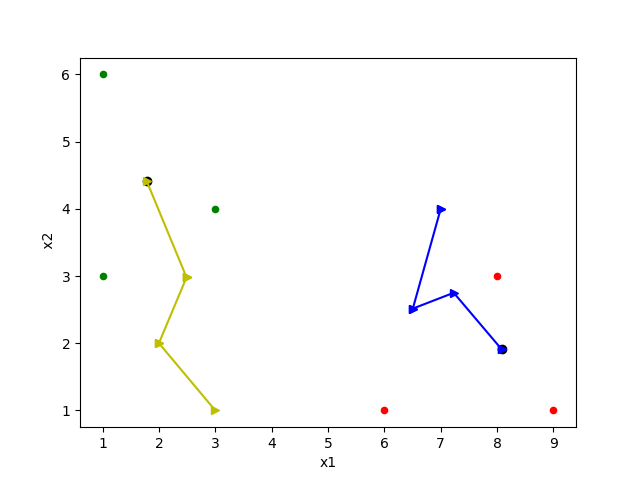
\includegraphics[height=10cm]{pic/lvq_weight_move.png}
	\caption{權重向量第一次迭代的移動路徑}
	\label{fig:lvq_weight_move}
\end{figure}

	      %
	\item 
		不斷重複以上2\char`\~ 5的步驟,直到設定的iteration到100爲止。圖\ref{fig:lvq_100_iteration}爲此資料集經過100次迭代的結果,可以發現權重向量移動的步伐因爲學習率的縮小,移動的越來越小,也因此它的值也漸漸固定不在改變,此外這兩個權重向量分別往兩個類別的群心點靠近。
\begin{figure}[h!]
	\centering
	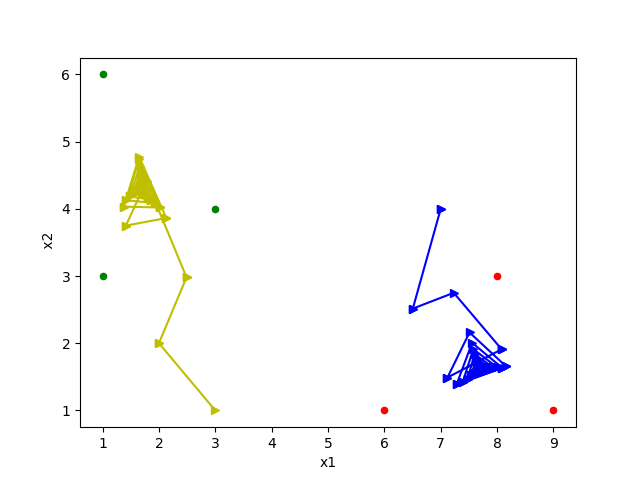
\includegraphics[height=10cm]{pic/lvq_100_iteration.png}
	\caption{經過100次迭代的結果}
	\label{fig:lvq_100_iteration}
\end{figure}

\end{enumerate}


\newpage

\section {結論}
從以上的實例可以發現這個演算法,其實蠻簡單的而且也易於理解,也因爲這個模型的參數較少,所以模型的訓練速度非常的快,以剛剛的資料集,在100次的迭代的情況下,訓練的時間不到15秒即可完成,所以這個演算法在資料集簡單的情況下,是能夠在短時間內訓練出一個不錯的模型。



%%RBF
\chapter{Radial Basis Function Neural Network}
\label{chapter:rbf}
\section{簡介}
Radial Basis Function Function(簡稱RBF)Network Work,圖\ref{fig:RbfNetwork}爲它的網路架構圖,其中有三層網路層,分別爲輸入、隱藏層與輸出層。在介紹這個演算法前我們先來看看圖\ref{fig:PerceptonProblem},在\ref{fig:PerceptonPa}、\ref{fig:PerceptonPb}情況下,我們都可以利用一條線兩種不同類別分割,但是遇到\ref{fig:PerceptonPc}的情況,卻不能用一條線將兩個類別分割出來,由此可見這就是Single Perceptron缺點。而RBF這個演算法的優勢就在於,可以解決了Single Perceptron在某些情況下線性不可切割的問題,可以將不可線性分割的資料集轉換到另一個維度如圖\ref{Fig:RbfTransfer}所示,使得轉換過的資料變成可線性分割的問題。
\begin{figure}[htbp]
	\centering
	\centerline{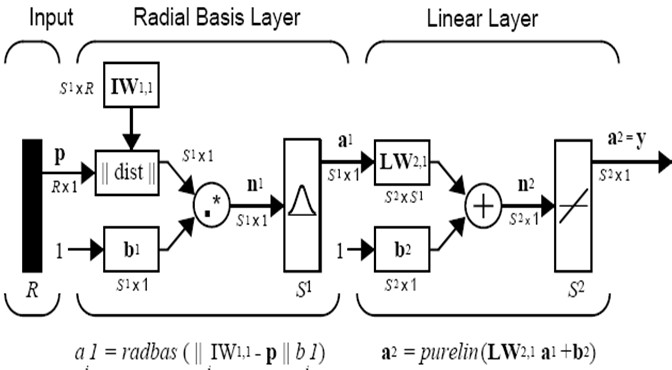
\includegraphics[width=10cm]{pic/rbf_struct.png}}
	\caption{RBF網路架構圖}
	\begin{minipage}{.7\linewidth}
		\footnotesize
		\emph{圖片來源:}取自Function approximation using artificial neural networks
	\end{minipage}
	\label{fig:RbfNetwork}
\end{figure}

\begin{figure}[H]
	\begin{center}
		\begin{tabular}{ccccccccccccc}
			\subfigure[]{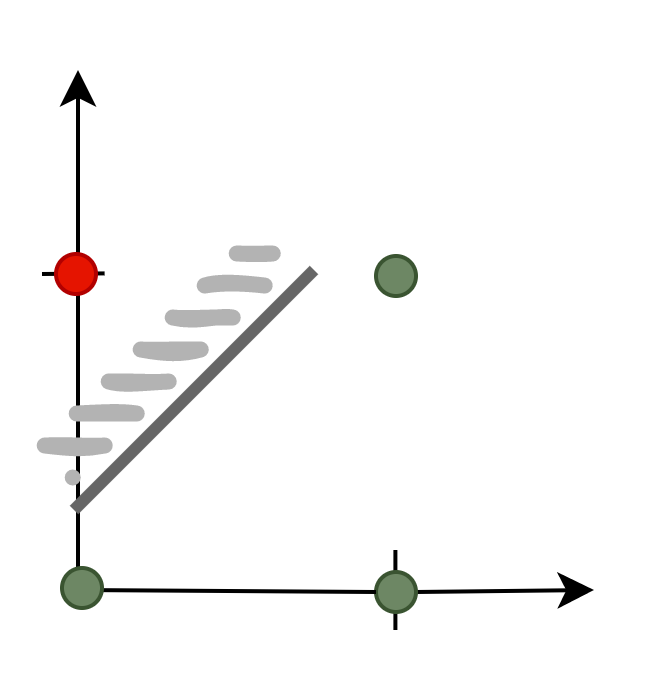
\includegraphics[height=4cm]{./pic/q9iv7T7i.png}\label{fig:PerceptonPa} } \par &
			\subfigure[]{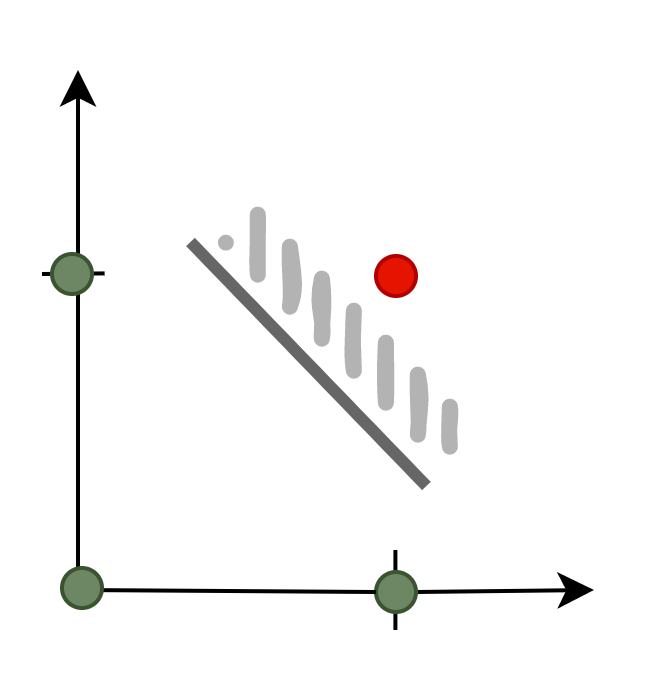
\includegraphics[height=4cm]{./pic/gQvdNdfq.png}\label{fig:PerceptonPb} } \par &
			\subfigure[]{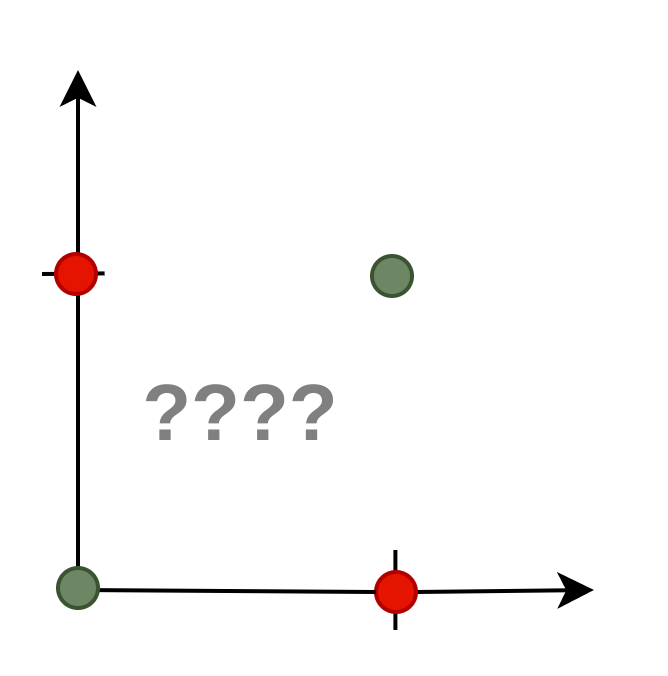
\includegraphics[height=4cm]{./pic/zLfLBK3B.png}\label{fig:PerceptonPc} } \par   \\
		\end{tabular}
		\caption{}
		\label{fig:PerceptonProblem}
	\end{center}
\end{figure}


%figure3
\begin{figure}[htbp!]
	\centering
	\subfigure[未轉換過的原資料]{
		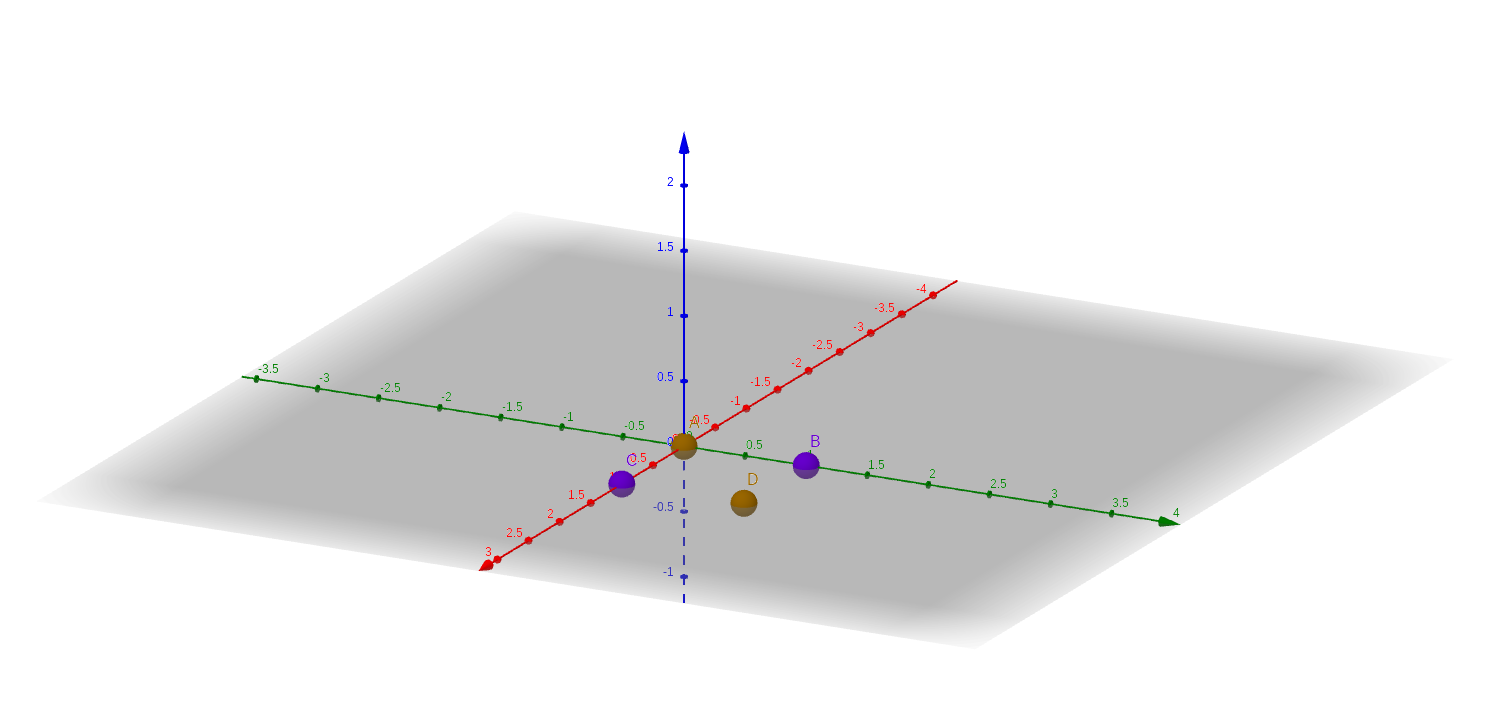
\includegraphics[width=10cm]{pic/Mxrc4anf.png}
		%\caption{fig1}
	}

	%	\quad
	\subfigure[經過轉換後的資料]{
		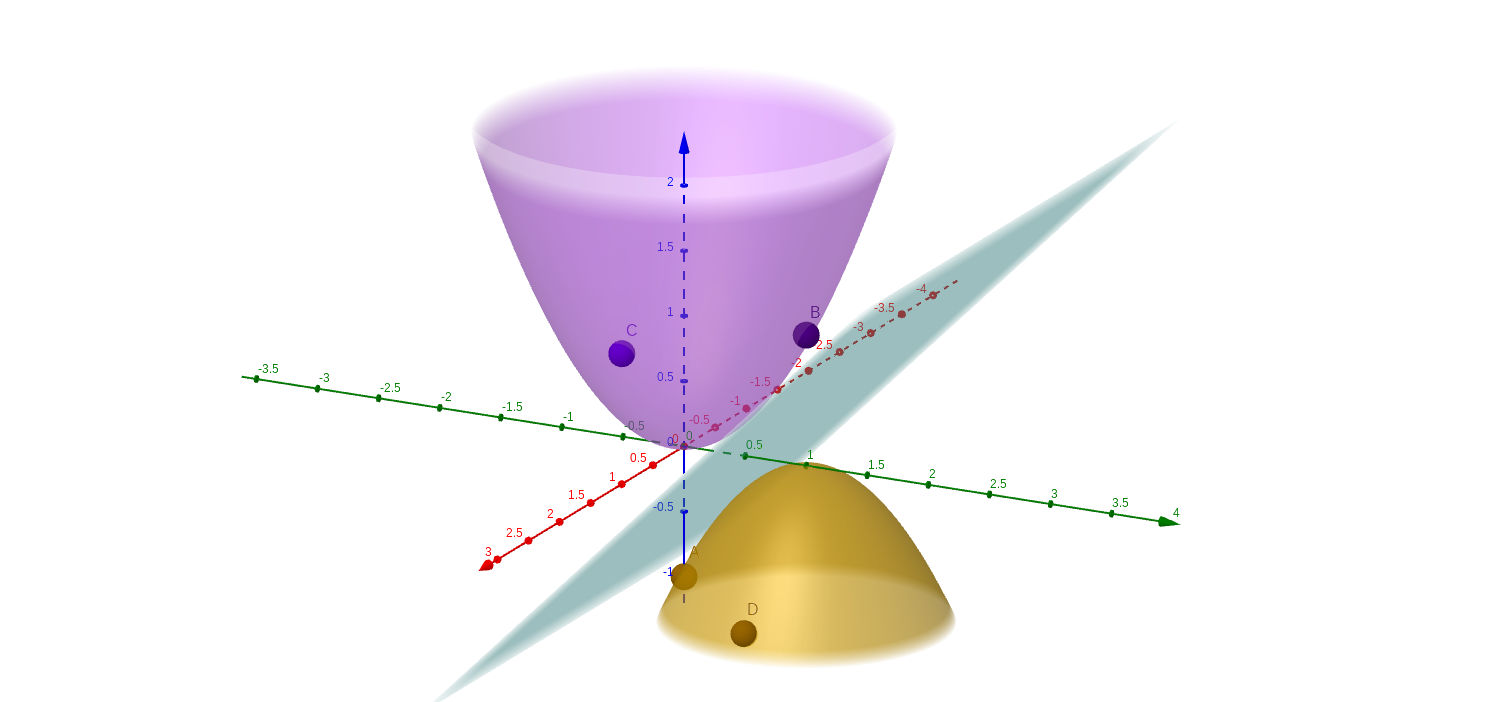
\includegraphics[width=10cm]{pic/JmIpjiQ2.png}
	\label{Fig:RbfTransfer}
	}

	\caption{資料轉換的示意圖}
\end{figure}



\section{Radial Basis Function}
前一小節提到RBF神經網路可以將資料轉換到另一個維度,而這個能將資料轉換到另一個維度的函數就是Hiden Layer中的 \(h(.)\),它也就是Radial Basis Function,以下舉個例子來說明它的運作:

\begin{itemize}
	\item

	      圖\ref{fig:RbfIntroductionNotTransfer}為一個一維的資料集,其中有藍色與橘色兩個類別,而我們的任務就是將這兩個類別分開。乍看之下僅用一條線將其分開,幾乎是不可能的任務,但是這也是我們限制在一個維度下才不能將其分離。



	      \begin{figure}[h]
		      \centering
		      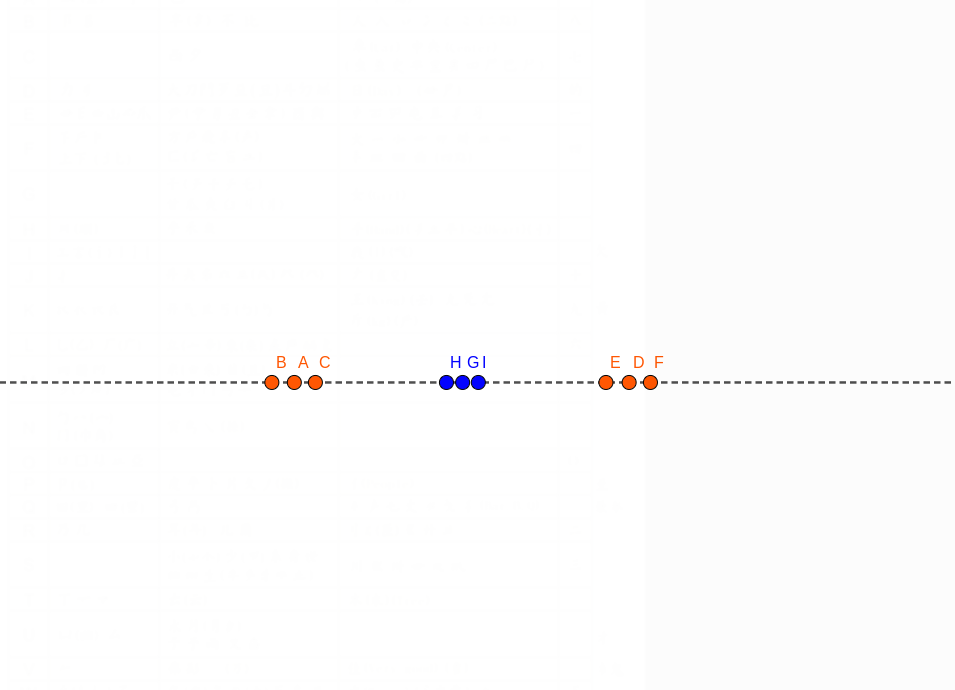
\includegraphics[height=6cm]{./pic/vM4xT9rm.png}
		      \caption{一維資料集}
		      \label{fig:RbfIntroductionNotTransfer}
	      \end{figure}

	\item
	      現在我們有一個 \(f(x)\) ,當我們的資料點經過這個函數的轉換,可以發現橘色點都向上移動,而藍色點都向下移動。經過函數轉換的結果後,我們要將這兩個類別進行切割就不難了。

	      \begin{figure}[h]
		      \centering
		      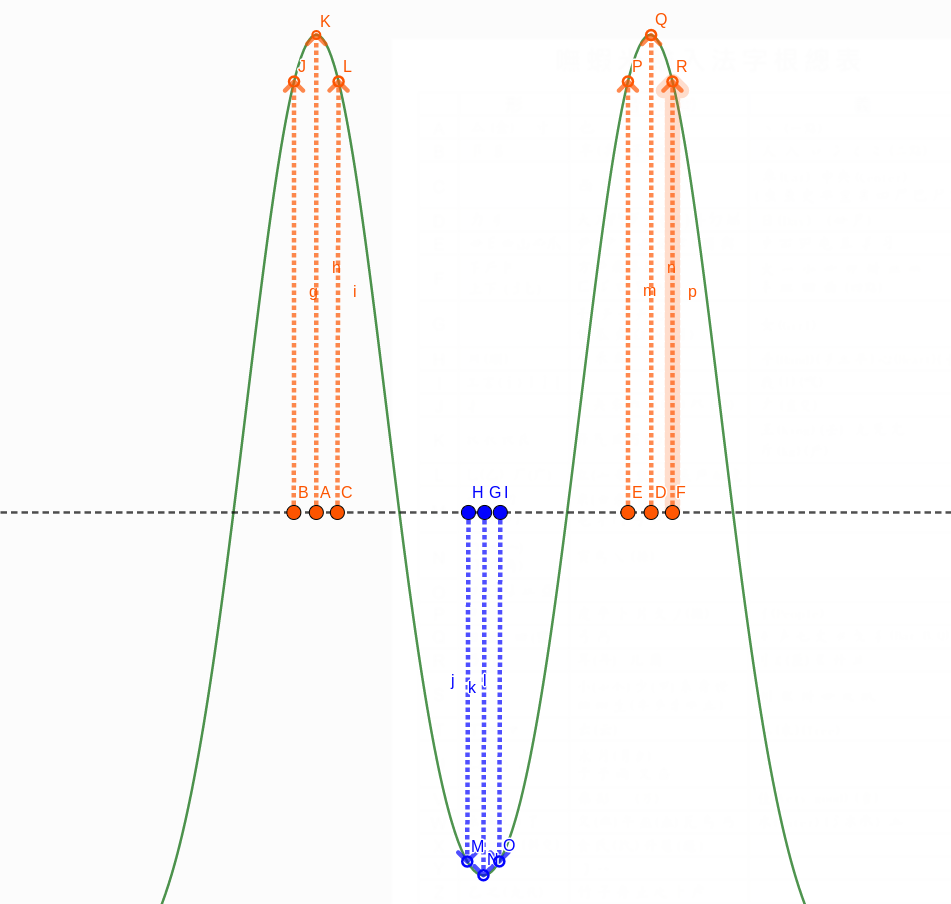
\includegraphics[width=6cm]{./pic/7VM3Lid5.png}
		      \caption{經過 \(f(x)\)轉換的結果 }
		      \label{fig:RbfWithFunction}
	      \end{figure}


	\item
	      而這個 \(f(x)\),其實是由3個不同的函數所組成在外加一個常數項所組成的,如圖\ref{fig:RbfFunctionAssemble}與\ref{eqn:RbfFunction}式所示。而其中的 \(h_1(x)\)、\(h_2(x)\)與\(h_3(x)\)就是就是 Radial Basis Function,藉由他們的組成可以將原本的資料集轉換到另一個維度。

	      \begin{equation}
		      \label{eqn:RbfFunction}
		      f(x)=w_1h_1(x)+w_2h_2(x)+w_3h_3(x)+b
	      \end{equation}

	      \begin{figure}[h]
		      \centering
		      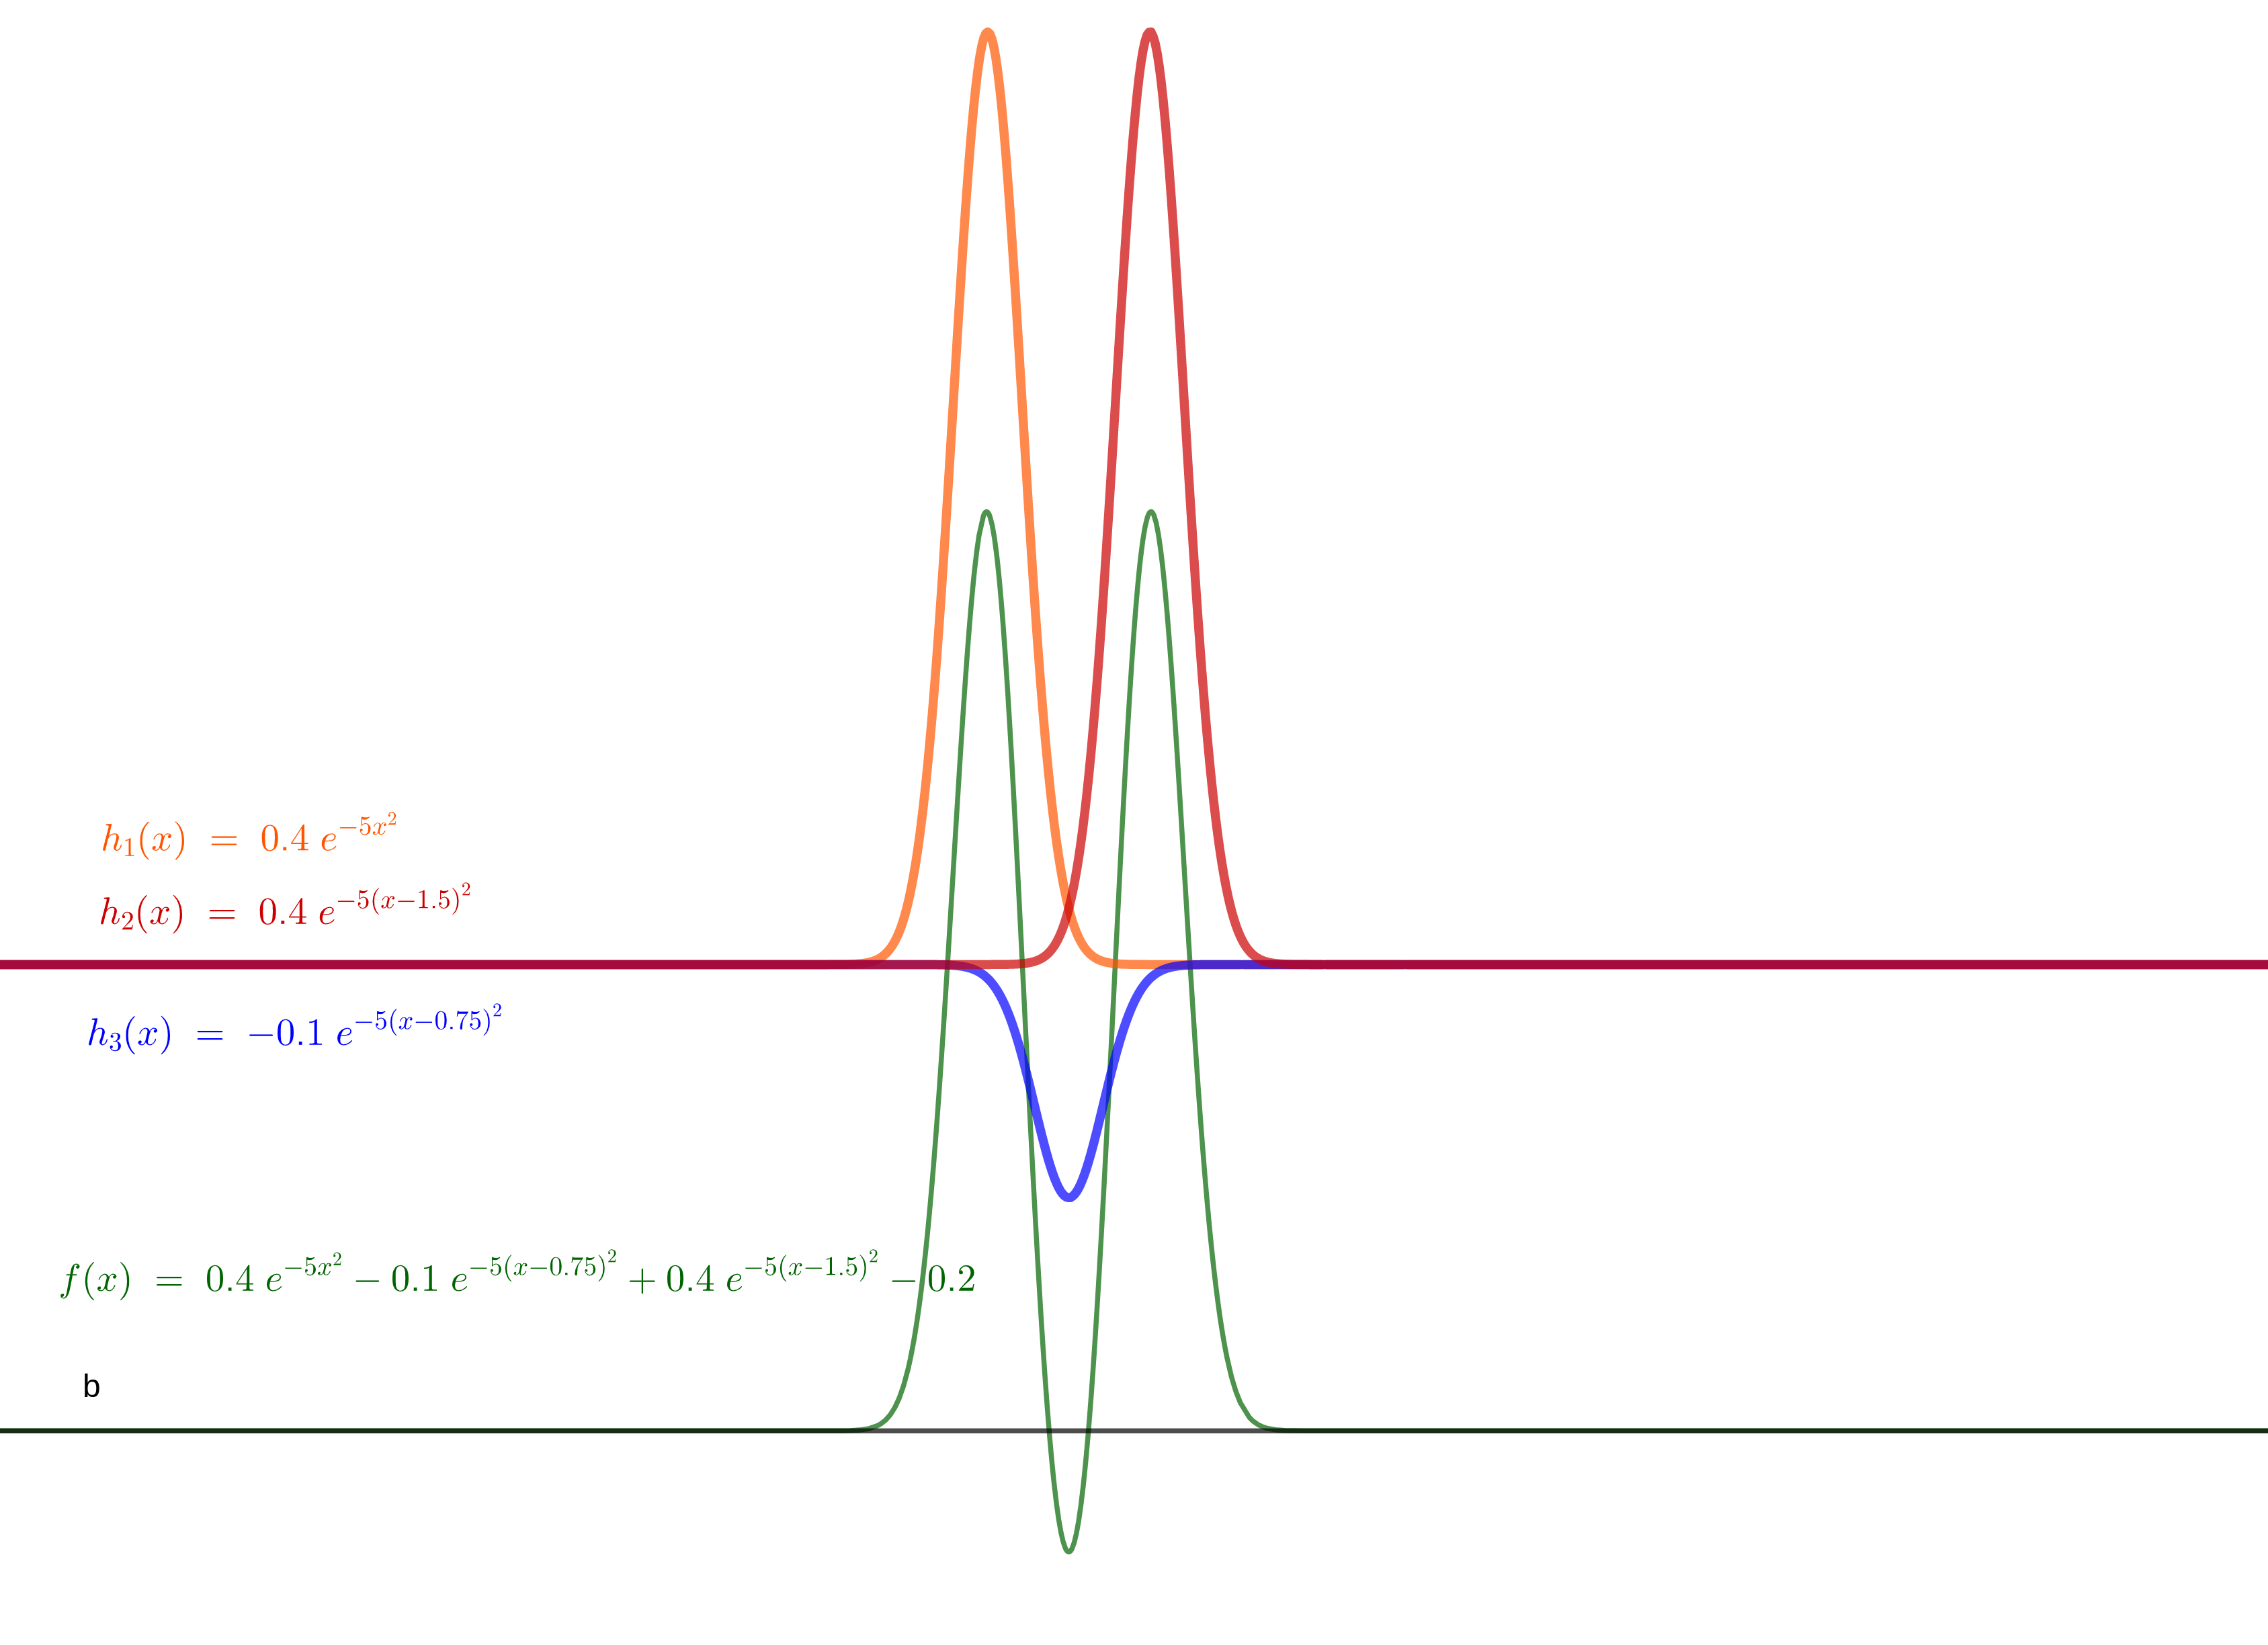
\includegraphics[height=6cm]{./pic/vtYD2no6.png}
		      \caption{\(f(x)\)的組成 }
		      \label{fig:RbfFunctionAssemble}
	      \end{figure}

	\item
	      Radial Basis Function(徑向基函數),之所以有個「Radial」,其實不難想像,就是跟中心點的距離有關係,所以通常這個函數會設定一個中心點,並將其他點與這個中心點的距離代入計算輸出結果。
	      式 \ref{eqn:RadialBasisFunction}與圖\ref{fig:RadialBasisFunction},爲一個中心點為1的高斯函數。
	      從圖中也能發現,離中心點越近可以得到越大值,代表與中心點越相關。反之離中心點越遠所得到的值就越小,代表與中心點越不相關。

	      \begin{equation}
		      \label{eqn:RadialBasisFunction}
		      h(x)= e^{-|1-x|^2}
	      \end{equation}

	      \begin{figure}[H]
		      \centering
		      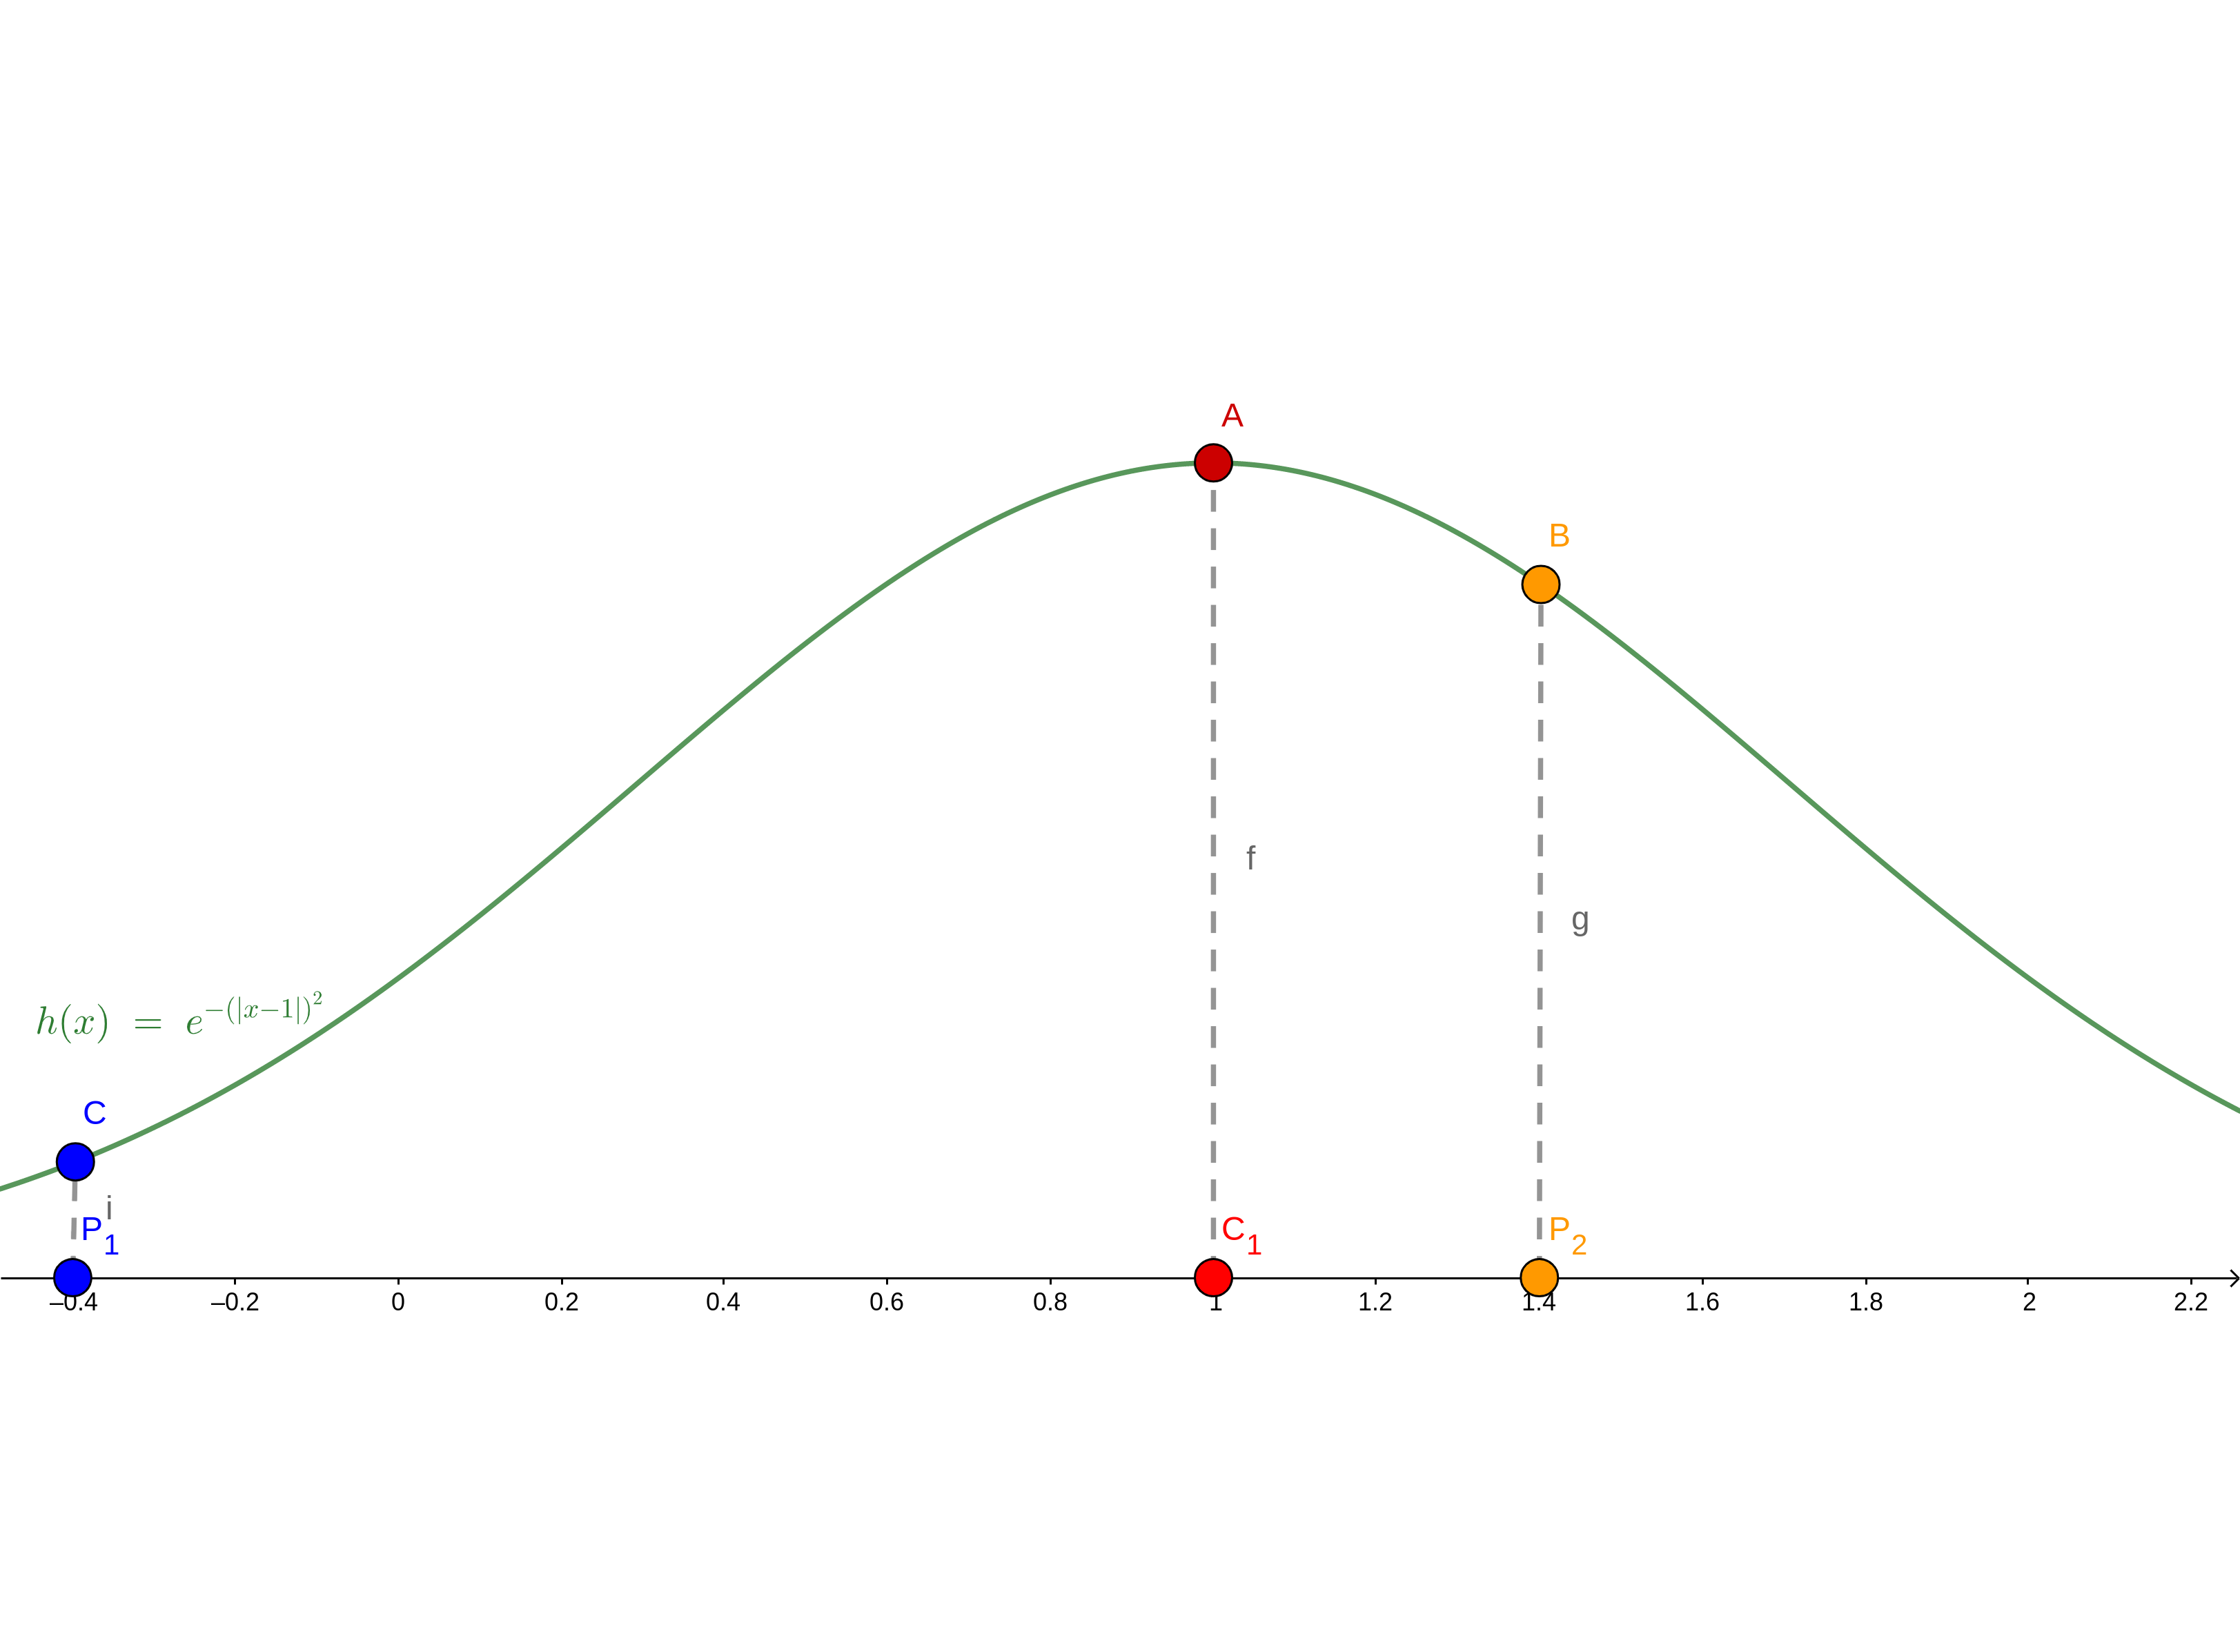
\includegraphics[height=6cm]{./pic/w0KFLczH.png}
		      \caption{}
		      \label{fig:RadialBasisFunction}
	      \end{figure}

\end{itemize}

當然Rail Basis Function有很多種,常見的如下表所示:
\\

\begin{table}[h!]
	\centering
	\label{tab:rbf_table}
	\begin{tabular}{ccc}
\toprule
  & RBF的名字 & 方程式 (\(r = ||\mathbf{C-X_i}||\) )   \\ 
\midrule
  & Gaussian Function  & \(h(r) = e^{-\varepsilon r}\)      \\ \\ 
  & Linear radial Function  & \(h(r) = r\)      \\ \\
  & Multiquadric   & \(h(r) = \sqrt{1+(\varepsilon r)^2}\)       \\ \\
  & Inverse quadric  &  \(h(r) = \frac{1}{1+(\varepsilon r)^2}\)     \\ \\ 
  & Inverse Multiquadric  &  \(h(r) = \frac{1}{\sqrt{1+(\varepsilon r)^2}}\)     \\
\bottomrule
\end{tabular}

	\caption{常見的Radial Basis Function}
\end{table}




%要被單行註解的文字。


\section{演算法參數定義與流程}




\subsection{參數定義}
\begin{itemize}
	\item
	      輸入向量,\(\mathbf{x} = (x_1,x_2,x_3,....,x_R)\),爲資料集中的其中一筆資料,輸入向量的 \(R\) 爲資料的特徵數量。
	      %
	\item
	      Radial Basis Layer權重,\(\mathbf{W^1} = [\mathbf{c_1,c_2,...,c_j,...c_{S_1}}]^T\),爲一個 \(S_1 \times R \)的矩陣,也就是前一節所介紹 Radial Basis Function中心點的集合,這邊的 \(S_1\)代表中心點的數量,而 \(\mathbf{c_j}\)為其中一個中心點 。
	      %
	\item
	      Radial Basis Function, 定義為\(\{h_1(x), h_2(x),...,h_j(x),....h_{S_1}(x) \}\)  。
	      這邊$h_j(x)=\phi(\mathbf{|c_j-x_i|})$。


	\item
	      輸出層權重, \(\mathbf{W^2}= [\mathbf{w_1,w_2,...,w_k,...,w_{S_2}}]^T\),為一個 \(S_2 \times S_1\) 的矩陣,這邊的 \(S_2\)代表輸出的類別數 。偏移向量為, \(\mathbf{b^2}=(b_1,b_2,....b_{S_2})\)。
	\item
	      輸出向量,\(\mathbf{y}= (y_1,y_2,...,y_k,...y_{S_2})\),其中式 \ref{eqn:RbfOutputLayer}為每個 \(\mathbf{y_k}\)的計算方式。其實仔細觀察可以發現式\ref{eqn:RbfOutputLayer}與式\ref{eqn:RbfFunction}所代表函意相同。

	      \begin{equation}
		      \label{eqn:RbfOutputLayer}
		      \mathbf{y_k}= f(x) = \sum_{i=1}^{S_1}w_{ik}\cdot h_i(x)+b_k
	      \end{equation}
	      %
	\item
	      實際類別, \(T\)。
\end{itemize}

\subsection{流程}

首先會先初始化 \(\textbf W^1\)  、 \(\textbf W^2\) 與 \(\mathbf{b^2}\) ,其中 \(\mathbf{W^1}\) 的中心點可以利用kmeans演算法得到,則\(\textbf W^2\) 與 \(\mathbf{b^2}\)可隨機生成。接著將所有的資料集進行訓練,利用自行選定的Radial Basis Function計算每筆 \(\mathbf x\)與每個中心點的 \(\{h_1,...,h_{S_1}\}\),以及計算其輸出結果 \(\mathbf{y}\),並透過最小平方法更新 \(\mathbf{W^2}\) 與 \(\mathbf{b}\) 的值。直到達到訓練條件。

\begin{figure}[H]
	\centering
		\resizebox{300pt}{400pt}{
		\begin{tikzpicture}[scale=1]
			\node[draw, rounded corners,align=center ]                        (start)   {初始化參數 \(\mathbf{W^1,W^2,b^2}\) };
			\node[draw,diamond, below=20pt of start,align = center]                        (input_x)  {訓練 \(\mathbf{x}\) 中的\\每一筆資料};
			\node[draw,  aspect=2, below=20pt of input_x, align = center]     (caculate_rbf_layer)  {計算Radial Basis Layer中的\\  \(h_1(x),h_2(x),...,h_j(x),..h_{S_1}(x)\)  };
			\node[draw,  aspect=2, below=20pt of caculate_rbf_layer, align = center]     (caculate_output_layer)  {計算Output Layer中的\\  \(y_1,y_2,...,y_k,..y_{S_2}\)  };
			\node[draw, below=20pt of caculate_output_layer,align = center]                   (update_output_weight)  {比對 \(y_k\)與 \(T\)\\ 接著利用最小平方法計算並更新 \(W^2\)   };
			\node[draw,diamond, below=20pt of update_output_weight,align = center]                         (end_detect)  {判斷是否\\達到結束條件};
			\node[draw, rounded corners, below=20pt of end_detect]  (end)     {End};

			\draw[->] (start)  --coordinate(le) (input_x);
			\draw[->] (input_x) --node[left]{Yes} (caculate_rbf_layer);
			\draw[->] (input_x.west) --node[above]{No}++(-60pt,0)|-(end_detect.west);
			\draw[->] (caculate_rbf_layer) -- (caculate_output_layer);
			\draw[->] (caculate_output_layer) -- (update_output_weight);
			\draw[->] (update_output_weight) -> (end_detect);
			\draw[->] (end_detect) -- node[left]{Yes}(end);
			\draw[->] (end_detect.east) --node[above]{No}++(250pt,0pt)|-(le) ;

		\end{tikzpicture}
	}

	\caption{演算法流程圖}
	\label{fig:AlogrithmWorkflow}
\end{figure}

\section {總結}
圖\ref{fig:RbfOutcome}為一個二維資料進行RBF Neural Network 訓練的結果,從圖中可以發現分別有紅藍兩類,黑色的*則代表各個中心點,經過訓練後可以在圖上畫出一個決策邊界。
從這個訓練結果可以明顯的看出RBF Neural Network這個演算法的優點,能順利將這種不可線性分割的資料集進行分類,又因為訓練的參數不多,所以短時間就能訓練出不錯的結果。

此外,在這個演算法中,中心點的數量與位置會影響訓練效果,數量太多會可能會導致訓練結果過擬合,數量太少則會導致訓練的結果不理想,而中心點的位置選的不好,即便數量對了,訓練的效果也可能會不好。




\begin{figure}[h]
	\centering
	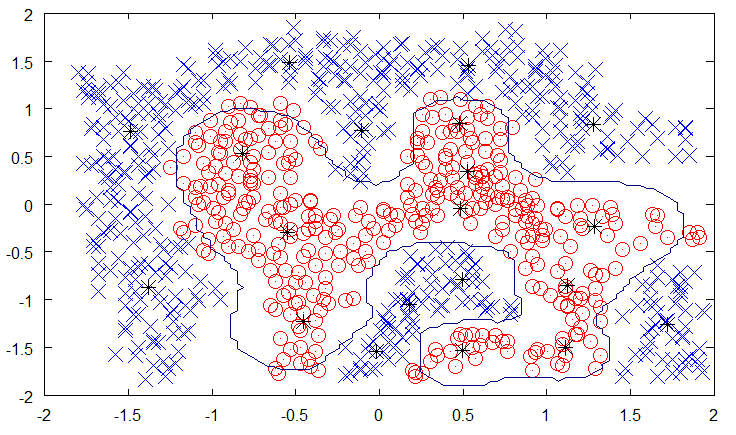
\includegraphics[height=5cm]{./pic/v35Qta6w.png}
	\caption{RBF Network以二維資料訓練的示意圖}

	\begin{minipage}{.7\linewidth}
		\centering
		\footnotesize
		\emph{圖片來源:}取自Radial Basis Function Network (RBFN) Tutorial
	\end{minipage}

	\label{fig:RbfOutcome}
\end{figure}


%%SVM
\chapter{Support Vector Machine }
\label{chapter:intro}
\section{SVM(Support Vector Machine)介紹}
SVM是一種線性分類器,可以處理線性分類問題如圖\ref{fig:Linear},同時卻也可以推展到解決非線性如圖\ref{fig:unkinear}的分割問題。將在低維度空間線性不可分的樣本映射到高維度空間去使 SVM 能在高維空間當中建構超平面如圖\ref{fig:overspace}或超平面集合,進而將原始數據進行分類,找到一個超平面將這些樣本做有效的切割,而這個超平面兩邊的樣本要盡可能地遠離這個超平面,為了將來多出新的資料時也能有效,而為了能針對不同類型的數據有個別的分類效果,
通常會選擇適當的核函式(kernel function)來使用,SVM 的主要如下公式:
\begin{equation}
	\label{equ:SVM}
	_{w,\delta_i}^{min}\frac{1}{2}W^TW+C\sum_{i=1}^{n}\delta_i
\end{equation}
其中 w 為超平面的法向量,$\delta_i$超平面的容忍邊界參數,值越大容忍範圍越大,
C 為調整容忍邊界參數的權重。




\begin{figure}[h]
	\centerline{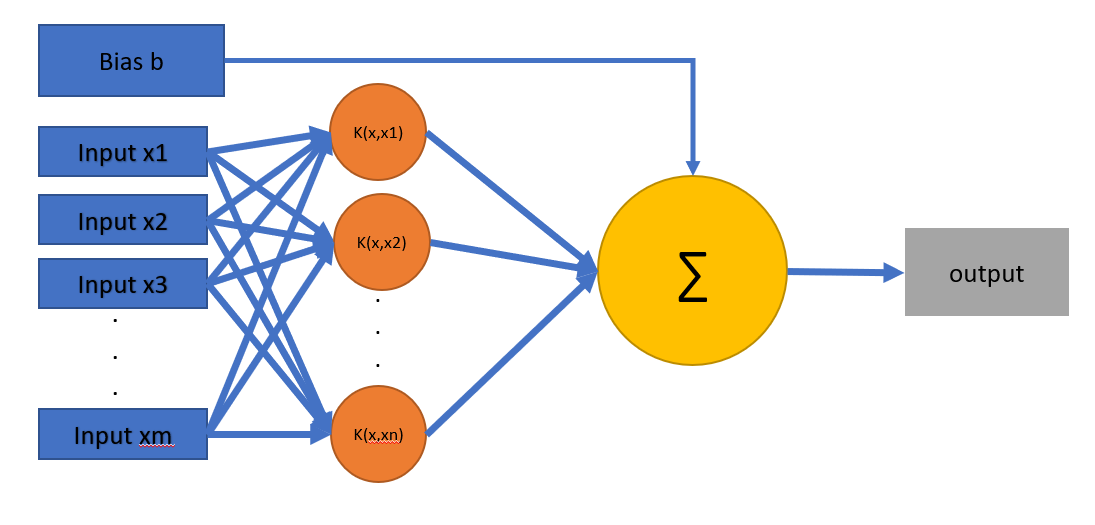
\includegraphics[height=8cm]{pic/SVM ar.PNG}}
	\caption{svm架構圖}
	\label{fig:svmar}
\end{figure}
\begin{figure}[h]
	\centerline{\includegraphics[height=8cm]{pic/SVML.png}}
	\caption{svm示意圖}
	\label{fig:svmar}
\end{figure}
\begin{figure}[H]
	\centerline{\includegraphics[height=5cm]{pic/linear.PNG}}
	\caption{線性可分示意圖}
	\label{fig:Linear}
\end{figure}
\begin{figure}[H]
	\centerline{\includegraphics[height=5cm]{pic/unlinear.PNG}}
	\caption{線性不可分示意圖}
	\label{fig:unkinear}
\end{figure}

\begin{figure}[H]
	\centerline{\includegraphics[height=5cm]{pic/over space.PNG}}
	\caption{超空間示意圖}
	\label{fig:overspace}
\end{figure}
\label{sec:background}

\section{核函數(kernel function)}
\begin{enumerate}
	\item
	      Linear Kernel
	      \begin{equation}
		      \label{Linear Kerne}
		      K(x,x')=x^Tx'
	      \end{equation}

	\item
	      Radial Basis Function Kernel
	      \begin{table}[h!]
		      \centering
		      \label{tab:rbf_table}
		      \begin{tabular}{ccc}
\toprule
  & RBF的名字 & 方程式 (\(r = ||\mathbf{C-X_i}||\) )   \\ 
\midrule
  & Gaussian Function  & \(h(r) = e^{-\varepsilon r}\)      \\ \\ 
  & Linear radial Function  & \(h(r) = r\)      \\ \\
  & Multiquadric   & \(h(r) = \sqrt{1+(\varepsilon r)^2}\)       \\ \\
  & Inverse quadric  &  \(h(r) = \frac{1}{1+(\varepsilon r)^2}\)     \\ \\ 
  & Inverse Multiquadric  &  \(h(r) = \frac{1}{\sqrt{1+(\varepsilon r)^2}}\)     \\
\bottomrule
\end{tabular}

		      \caption{常見的Radial Basis Function}
	      \end{table}
	\item
	      Sigmoid Kernel
	      \begin{equation}
		      \label{Sigmoid Kerne}
		      S(t)=\frac{1}{1+e^{-t}}
	      \end{equation}


\end{enumerate}

\begin{figure}[H]
	\centerline{\includegraphics[height=5cm]{pic/linear kernel.png}}
	\caption{linear kernel示意圖}
	\label{fig:linear kernel}

	\centerline{\includegraphics[height=5cm]{pic/Radial Basis Function Kernel.png}}
	\caption{Radial Basis Function Kernel示意圖}
	\label{fig:Radial Basis}

	\centerline{\includegraphics[height=5cm]{pic/Sigmoid Kernel.png}}
	\caption{Sigmoid Kernel示意圖}
	\label{Sigmoid Kernel}
\end{figure}



%%  文獻
%\bibliographystyle{IEEEtran}
%    \bibliographystyle{plain}
%    \bibliographystyle{apa}
%    \bibliographystyle{apacite}\renewcommand{\bibname}{參考文獻}
%\bibliography{citations/ref_title1,citations/ref_title2}

%%%%%%%%%%%%%%%%---------- 附錄
%\begin{appendices}
%	\appendix
%	%        \noappendicestocpagenum
%	\titleformat{\chapter}[display]{\center\LARGE\sf}{附錄 \thechapter}{0.2cm}{}  % 設計附錄標題式樣,標題置中
%	\chapter{相關公式}
\label{chapter:appendix_eq}

    質能互換公式為\eqref{eq:mass_energy_equivalence}。
    \begin{equation}\label{eq:mass_energy_equivalence}
      E=MC^2
    \end{equation}

 %% appendix-A
%	\chapter{相關表格}
\label{chapter:appendix_tables}

    ○○○對應表為\ref{tab:mytitle2}。
    \begin{table}[htbp]
        \centering
        \caption{表格標題2}
        \label{tab:mytitle2}
        % Table generated by Excel2LaTeX from sheet '工作表1'
\begin{tabular}{rrr}
\toprule
Number & Class & Values \\
\midrule
1     & A     & 21 \\
2     & B     & 854 \\
3     & C     & 458 \\
4     & D     & 87 \\
5     & E     & 1654 \\
6     & F     & 978 \\
7     & G     & 23 \\
8     & H     & 746 \\
9     & I     & 278 \\
\bottomrule
\end{tabular}%

    \end{table}

 %% appendix-A
%\end{appendices}

%===============================================================
\end{document}
